% ========================================
% Document Class and Package Setup
% ========================================
\documentclass[%
 reprint, amsmath,amssymb, aps, prb, ]{revtex4-2}
\usepackage{graphicx}
\usepackage{bm}
\usepackage{physics}
\usepackage[colorlinks=true,
            linkcolor=blue, filecolor=blue, urlcolor=blue, citecolor=blue]{hyperref}
\usepackage{caption}
\captionsetup[figure]{
    justification=raggedright, labelfont={bf}, name={Fig.}, labelsep=period }
\captionsetup[table]{
    labelfont={bf}, name={Table}, labelsep=period }
\numberwithin{equation}{section}
\tolerance=1000
\emergencystretch=1em
\hyphenpenalty=3000
\exhyphenpenalty=3000
\flushbottom
\usepackage[final]{microtype}
\usepackage{ragged2e}  % for \justifying command
\usepackage{booktabs}
\usepackage{enumitem}
% Theorem environment
\usepackage{amsthm}
\newtheorem{theorem}{Theorem}[section]
\newtheorem{hypothesis}{Hypothesis}[section]
\newtheorem{proposition}{Proposition}[section]
% --- paragraph heading: run-in italic with extra top skip for block readability ---
\makeatletter
\renewcommand\paragraph{%
  \@startsection{paragraph}{4}{\z@}%
    {3mm \@plus 1ex \@minus .2ex}
    {-1em}
    {\normalfont\normalsize\itshape}}
\makeatother
% Code listings with syntax highlighting
\usepackage{listings}
\usepackage{xcolor}
\definecolor{backcolour}{rgb}{0.96,0.97,0.98}
\definecolor{deepblue}{rgb}{0,0,0.5}
\definecolor{deepgreen}{rgb}{0,0.5,0.3}
\definecolor{deepgray}{rgb}{0.4,0.4,0.4}
\definecolor{stringcolor}{rgb}{0.2,0.4,0.6}
\lstdefinestyle{pythonstyle}{
    backgroundcolor=\color{backcolour}, commentstyle=\color{deepgreen}\itshape, keywordstyle=\color{deepblue}\bfseries, numberstyle=\tiny\color{deepgray}, stringstyle=\color{stringcolor}, basicstyle=\ttfamily\footnotesize, breakatwhitespace=false, breaklines=true, captionpos=b, keepspaces=true, numbers=left, numbersep=5pt, showspaces=false, showstringspaces=false, showtabs=false, tabsize=2, language=Python, frame=single, rulecolor=\color{deepgray} }
\lstset{style=pythonstyle}
% Internal phase notation
\newcommand{\iphase}{\theta}  % internal geometric phase = ωt/2
\usepackage{tikz}
\usetikzlibrary{arrows.meta, calc, 3d, shadings, positioning, decorations.pathmorphing}
% --- Custom Macros ---
\newcommand{\omZB}{\omega_{\text{ZB}}}
\newcommand{\EphS}{E_{\text{ph}}}
\newcommand{\Egrad}{\Delta E_{\text{AB}}}
% Fundamental 1-form
% Field strength 2-form
\newcommand{\FF}{\mathbf{F}}
% Open Wilson line
\newcommand{\WL}{\mathcal{W}}
% Hodge dual
\newcommand{\hodge}{\star}

% ========================================
% Document Begin
% ========================================
\begin{document}

% ========================================
% Title, Author, and Date
% ========================================
\title{A Dual-Model Deliberation Record on the Spin-2 Sector of the 0-Sphere Model:\\ Cross-Verification Dialogue between Claude Opus 4.8 and Claude Fable 5}

\author{Satoshi Hanamura}
\email{hana.tensor@gmail.com}
\date{July 5, 2026 (archival revision: July 19, 2026)}

% ========================================
% Abstract
% ========================================
\begin{abstract}
This document is not a research paper but an archival deliberation record with a prospecting purpose.
In early July 2026 the author charged two large language models --- Claude Opus 4.8 and Claude Fable 5 (Anthropic) --- with a single theme: starting from the published 0-Sphere model series, excavate the points at which the theory can be deepened and identify where the groundwork for the next papers should be laid, taking the gravitational-mediator line of the series (Papers \#49--\#59) as the designated sector.
The two models examined the sector in parallel sessions under the author's arbitration, each model checking the other's claims against the source manuscripts.
The deliberation produced six citable outcomes: (i) the separation of the ``spin-2 problem'' into two independent problems --- the mass-quadrupole rank-2 structure (resolved by conservation laws but outsourced to general relativity) and the Berry-curvature--Riemann correspondence (untouched by Paper \#59, and formulated as the Berry--Synge--Bonnet--Myers triangle programme of Paper \#60); (ii) a candidate answer to open task (I) of Paper \#58, in which the fixed chirality of Paper \#50, combined with the momentum reversal of the phase-stable fragment pair, yields an automatically traceless helicity-$\pm 2$ tensor structure $\varepsilon_{+\mu}\varepsilon_{+\nu}$ and a two-particle axial angular momentum $J_x=\pm2$ consistent with the Landau--Yang selection rule; (iii) a concrete form of the escape route from the Weinberg--Witten theorem, in which the back-to-back pair is a massive $J=2$ source configuration rather than a massless composite graviton; (iv) the demarcation of the boundary between task (I) (source-side tensor structure) and open problem O3 (massless radiation from the emergent metric); (v) a reformulation of open task (C) of Paper \#59 as a supply obligation for the $h_{\mu\nu}T^{\mu\nu}_{\mathrm{EM}}$ coupling channel; and (vi) three Corrections Log entries against Papers \#58 and \#59.
These outcomes are consolidated into seven candidate directions for future papers, with their prerequisites and dependencies mapped.
Equally important, the record preserves --- symmetrically and without attenuation --- the errors, retractions, and corrections-of-corrections committed by both models, as a working specimen of dual-model verification.
The document is designed to be read both by human readers and by future reasoning sessions, alongside a comprehensive review of the series, as the map from which the next move is chosen.
\end{abstract}

\maketitle

% ========================================
% Section 1: Introduction and Method
% ========================================
\section{Introduction and Method}
\label{sec:intro}

% ----------------------------------------
% Subsection 1.1: Purpose of this record
% ----------------------------------------
\subsection{Purpose of this record}

The 0-Sphere model series has been developed since 2018 as a single-author research program, with large language models used in supportive roles that are declared in the acknowledgments of each paper. The present document records a different use: a session in which two distinct models, Claude Opus 4.8 and Claude Fable 5, were not assistants but named dialogue participants, charged by the author with a prospecting theme --- to excavate, from the published series, the points at which the theory can be deepened, and to identify where the groundwork for the next papers should be laid. The author relayed each model's comments to the other and intervened at turning points to guide the direction of the deliberation.

This record is deposited on Zenodo as \#66 of the series --- an archival deliberation record, distinct in genre from the research papers of the corpus. It is not submitted for peer review and makes no claim to the standards of a journal article. Its purpose is threefold. First, it fixes the priority and provenance of several substantive results (Sec.~\ref{sec:ledger}) that subsequent papers in the series may cite by DOI. Second, it consolidates those results into an explicit map of candidate directions for future papers (Sec.~\ref{sec:stones}), which is the deliverable the theme asked for. Third, it preserves the \emph{method}: the session produced multiple rounds of mutual error detection, retraction, and correction-of-correction, and this process --- which vanishes from a results-only paper --- is itself worth archiving, both for the transparency policy of the series and as a specimen of dual-model verification practice.

A remark on the intended readership. This document is written to be legible to a human reader with a graduate-level physics background, but it is equally written to be \emph{loaded}: the author intends to supply it, together with a comprehensive review of the series, to future reasoning sessions as the prompt from which the next move is explored. Appendix~\ref{app:future} gives explicit reading instructions for that use. Appendix~\ref{app:checks} reproduces, without skipped steps, the explicit arithmetic behind every numerical and algebraic verification quoted in this record; it is addressed to readers new to the material, and doubles as a machine-checkable restatement of the session's verification norms. Appendix~\ref{app:glossary} provides a glossary --- standard terms, 0-Sphere terms, and the record's label systems --- pitched at a reader beginning graduate study.

% ----------------------------------------
% Subsection 1.2: Method: dual-model cross-verification
% ----------------------------------------
\subsection{Method: dual-model cross-verification}

The session proceeded as follows. The author posed the theme (Sec.~\ref{sec:theme}) to Claude Fable 5; Fable 5's opening assessment was relayed by the author to a parallel session with Claude Opus 4.8, whose response was relayed back, and so on, for ten exchanges. Source manuscripts (Papers \#10, \#49, \#50, \#51, \#52, \#58, \#59 \cite{hanamura10,hanamura49,hanamura50,hanamura51,hanamura52,hanamura58,hanamura59}) were supplied by the author as attachments whenever either model requested them. Both models were bound by the same session rules: verify every equation numerically; collate every line-number citation against the source before relying on it; re-run every reported text search before relying on its result; and treat nothing --- including the other model's claims and the author's own framing --- as authoritative.

Two properties of the resulting dialogue deserve emphasis. First, the two models disagreed, and their disagreements were resolved by collation against the sources, not by deference. Second, both models committed errors, and both retracted them when confronted with the sources. The full symmetric record of these errors is given in Table~\ref{tab:errors}; the editorial principle governing this record is stated next.

% ----------------------------------------
% Subsection 1.3: Editorial policy and attribution
% ----------------------------------------
\subsection{Editorial policy and attribution}

\paragraph{Reconstructed minutes, not verbatim transcript.} The deliberation was conducted in Japanese. This record is a reconstructed English-language account of the exchanges, composed by Claude Fable 5 and reviewed by the author. Where an agent's phrasing carried weight, it is quoted in translation and marked as such.

\paragraph{Symmetric recording of errors.} Mutual corrections are recorded symmetrically; neither agent's errors are attenuated. This principle was stipulated by Opus 4.8 as a condition of the archive --- in translation: ``a record of two-agent verification loses its value the moment one side dilutes its own errors'' --- and accepted without reservation by Fable 5 and the author.

\paragraph{Attribution.} The author of this record is Satoshi Hanamura alone. Claude Opus 4.8 and Claude Fable 5 (both Anthropic) participated as named dialogue agents; their roles are described in the body of this record. All physical judgments and all canonical decisions concerning the 0-Sphere model rest with the author; the two models functioned as verification agents. Canonical decisions that remained open at the close of the session are listed in Sec.~\ref{sec:deferred} and are explicitly \emph{not} decided by this record.

% ========================================
% Section 2: The Theme and the Starting Position
% ========================================
\section{The Theme and the Starting Position}
\label{sec:theme}

The author's charge to the two models, paraphrased from its original statement, was: \emph{from the papers I have written, find where the theory can be deepened and extended; identify where the stones for the next papers should be placed.} The designated sector for this session was the gravitational-mediator line of the series --- Papers \#49 through \#59 --- which develops the proposal that gravitational interaction is mediated by photon-sphere fragments ejected from the internal two-kernel dynamics of the electron \cite{hanamura49}, culminating in the phase-stable pair-emission mechanism of Paper \#58 \cite{hanamura58} and the proton-trapped quadrupole radiation of Paper \#59 \cite{hanamura59}.

The central open question of that sector, taken as the starting position, is representation-theoretic. A spin-2 mediator demands a symmetric traceless rank-2 tensor structure, which under the Lorentz group belongs to the $(1,1)$ representation; the natural curvature object of the series' line-integral program --- the field-strength or Berry-curvature 2-form $F_{\mu\nu}$ --- is antisymmetric and belongs to $(1,0)\oplus(0,1)$. No Lorentz-covariant linear map connects the two, so the search for an ``antisymmetric-to-symmetric conversion'' is closed by representation theory before it begins. The question the session inherited is therefore: \emph{by what route, if any, does the corpus actually obtain a rank-2 symmetric object --- and is that route load-bearing?}

Beneath the designated sector lies a foundational trilogy of the series that the deliberation presupposes throughout, and which this record makes explicit here. Paper \#29 \cite{hanamura29} establishes that a spinorial connection is embedded along the thermal geodesic by relativistic kinematics alone: the line integral $\tfrac{1}{2}\int(\mathbf a\times\mathbf v)\,d\tau$ of the Thomas-precession connection accumulates $2\pi$ of internal phase per one-way kernel traversal --- in two lobes of $\pi$ each, separated by the midpoint where the acceleration vanishes --- and the operative geometric object is the line integral of a connection, not the curvature of the spatial path nor the integration of a fiber bundle. Paper \#30 \cite{hanamura30} declares the program's reading of gravitation: conservation laws arise from connection-based phase accumulation, stress--energy is a derived rather than fundamental quantity, and the Einstein field equation functions not as a generative dynamical law but as an a posteriori global consistency condition --- a \emph{geometric checksum} --- verifying that accumulated phase along worldlines remains self-coherent. Paper \#31 \cite{hanamura31} generalizes this into the program's ordering principle: physical observables are holonomies of connections along histories --- the Aharonov--Bohm phase, the Berry phase, Wilson loops, and the two-kernel energy transport as instances of one class --- with local curvature a derived descriptor of infinitesimal transport. This trilogy is the standard against which several of the session's findings acquire their weight: the outsourcing verdict of Table~\ref{tab:split}, the two-metric problem, and candidate directions D2, D3, and D6 of Sec.~\ref{sec:stones} are all, in the end, statements about whether the gravitational sector of \#49--\#59 lives up to the hierarchy the trilogy declares.

Fable 5's opening move reframed the question. For a single object the representation gap is final; for a \emph{pair} it is not, because the tensor product of two vector representations decomposes as $1\otimes1=0\oplus1\oplus2$, whose symmetric traceless part is spin-2 --- the structure exploited, in standard physics, by the double-copy relations between gauge and gravity amplitudes \cite{klt,bcj}. Since Paper \#58's mechanism ejects fragments in pairs, the question becomes whether the corpus supplies \emph{two independent vector polarizations}, and the opening move simultaneously flagged a tension: the predecessor mechanism of Paper \#49 describes single-fragment ejection per de-excitation. The deliberation recorded in Sec.~\ref{sec:record} is, in essence, the collision of this opening move with the actual texts of Papers \#58 and \#59, and the reconstruction that followed. A second opening proposal --- that the type of the interior field equation of the photon sphere decides the ontological primacy of line integrals versus continuous fields --- was set aside once the spin-2 material arrived, and reappears as candidate direction D6 in Sec.~\ref{sec:stones}.

% ========================================
% Section 3: Chronological Record of the Deliberation
% ========================================
\section{Chronological Record of the Deliberation}
\label{sec:record}

Figure~\ref{fig:flow} gives the overall flow. The exchanges are numbered E1--E10; corrections are marked where one agent's claim was struck by the other's collation.

\begin{figure*}[t!]
\centering
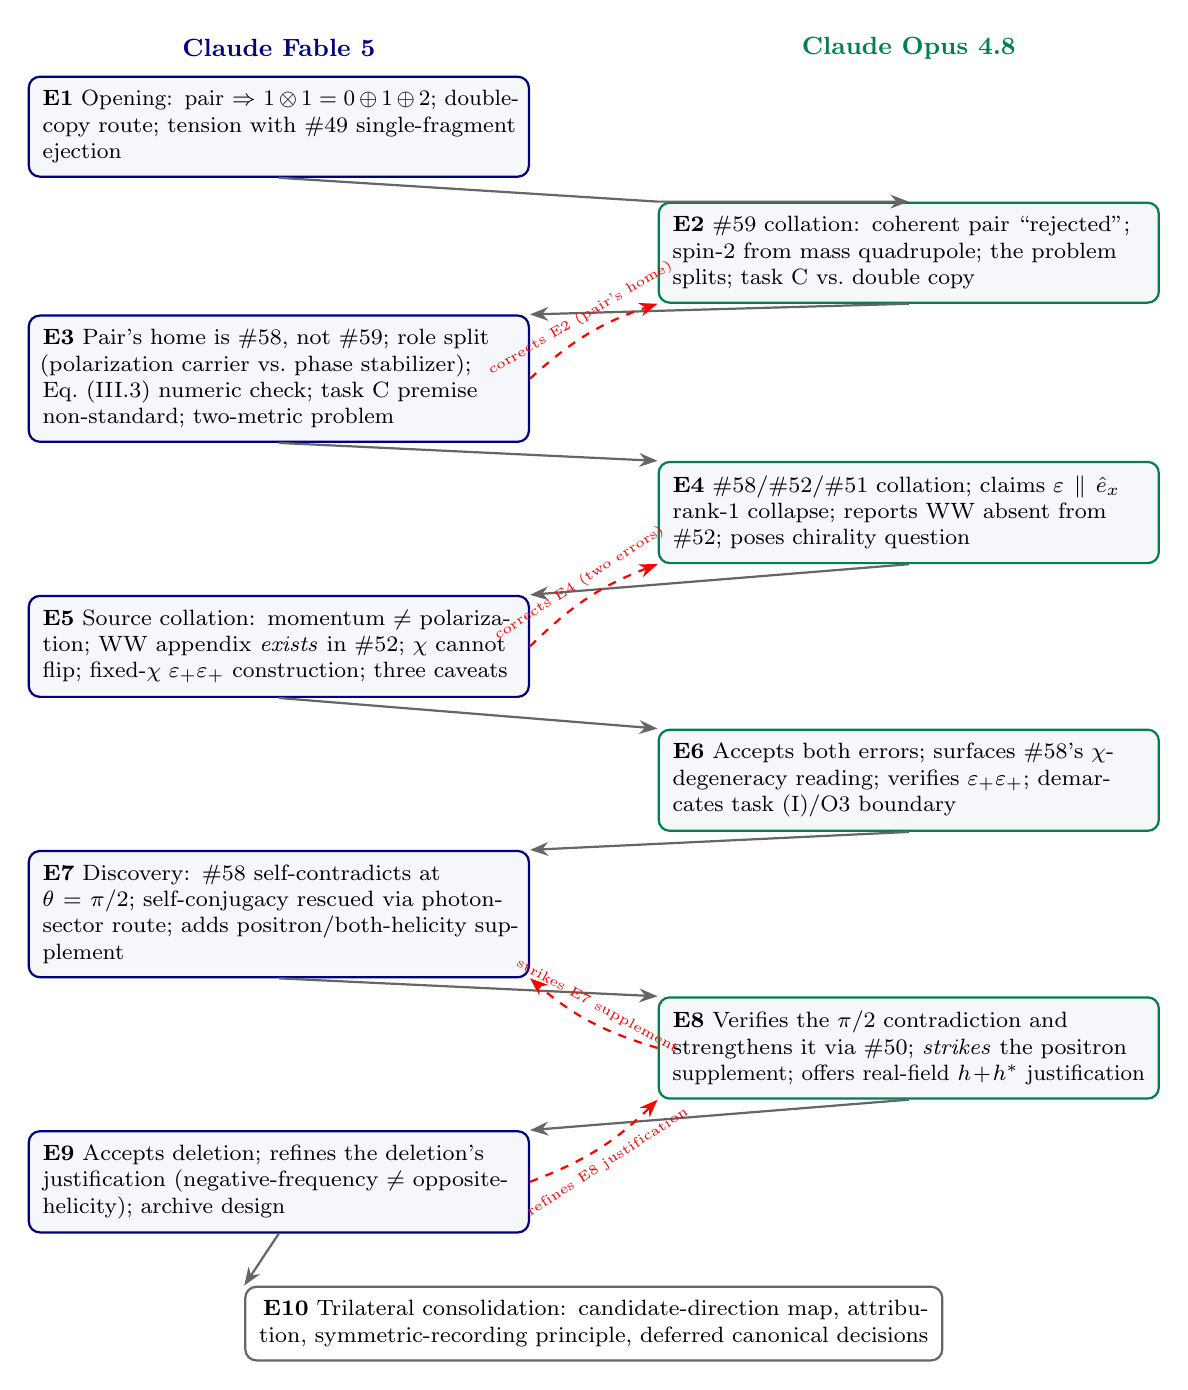
\begin{tikzpicture}[
  fnode/.style={draw=deepblue, thick, rounded corners, fill=backcolour, text width=6.0cm, align=left, font=\footnotesize, inner sep=5pt},
  onode/.style={draw=deepgreen, thick, rounded corners, fill=backcolour, text width=6.0cm, align=left, font=\footnotesize, inner sep=5pt},
  cnode/.style={draw=deepgray, thick, rounded corners, fill=white, text width=8.5cm, align=center, font=\footnotesize, inner sep=5pt},
  corr/.style={-{Stealth}, red, dashed, thick},
  flow/.style={-{Stealth}, deepgray, thick}
]
\node[font=\small\bfseries, text=deepblue] (fhead) at (-4.0, 1.0) {Claude Fable 5};
\node[font=\small\bfseries, text=deepgreen] (ohead) at (4.0, 1.0) {Claude Opus 4.8};
\node[fnode] (e1) at (-4.0, 0)   {\textbf{E1} Opening: pair $\Rightarrow$ $1\otimes1=0\oplus1\oplus2$; double-copy route; tension with \#49 single-fragment ejection};
\node[onode] (e2) at (4.0, -1.6) {\textbf{E2} \#59 collation: coherent pair ``rejected''; spin-2 from mass quadrupole; the problem splits; task C vs.\ double copy};
\node[fnode] (e3) at (-4.0, -3.2) {\textbf{E3} Pair's home is \#58, not \#59; role split (polarization carrier vs.\ phase stabilizer); Eq.~(III.3) numeric check; task C premise non-standard; two-metric problem};
\node[onode] (e4) at (4.0, -4.9) {\textbf{E4} \#58/\#52/\#51 collation; claims $\varepsilon\parallel\hat e_x$ rank-1 collapse; reports WW absent from \#52; poses chirality question};
\node[fnode] (e5) at (-4.0, -6.6) {\textbf{E5} Source collation: momentum $\neq$ polarization; WW appendix \emph{exists} in \#52; $\chi$ cannot flip; fixed-$\chi$ $\varepsilon_+\varepsilon_+$ construction; three caveats};
\node[onode] (e6) at (4.0, -8.3) {\textbf{E6} Accepts both errors; surfaces \#58's $\chi$-degeneracy reading; verifies $\varepsilon_+\varepsilon_+$; demarcates task (I)/O3 boundary};
\node[fnode] (e7) at (-4.0, -10.0) {\textbf{E7} Discovery: \#58 self-contradicts at $\iphase=\pi/2$; self-conjugacy rescued via photon-sector route; adds positron/both-helicity supplement};
\node[onode] (e8) at (4.0, -11.7) {\textbf{E8} Verifies the $\pi/2$ contradiction and strengthens it via \#50; \emph{strikes} the positron supplement; offers real-field $h+h^{*}$ justification};
\node[fnode] (e9) at (-4.0, -13.4) {\textbf{E9} Accepts deletion; refines the deletion's justification (negative-frequency $\neq$ opposite-helicity); archive design};
\node[cnode] (e10) at (0, -15.2) {\textbf{E10} Trilateral consolidation: candidate-direction map, attribution, symmetric-recording principle, deferred canonical decisions};
\draw[flow] (e1.south) -- (e2.west|-e2.north) -- (e2.north);
\draw[flow] (e2.south) -- (e3.north east);
\draw[flow] (e3.south) -- (e4.north west);
\draw[flow] (e4.south) -- (e5.north east);
\draw[flow] (e5.south) -- (e6.north west);
\draw[flow] (e6.south) -- (e7.north east);
\draw[flow] (e7.south) -- (e8.north west);
\draw[flow] (e8.south) -- (e9.north east);
\draw[flow] (e9.south) -- (e10.north west);
\draw[corr] (e3.east) to[bend left=12] node[midway, above, sloped, font=\tiny\color{red}] {corrects E2 (pair's home)} (e2.south west);
\draw[corr] (e5.east) to[bend left=12] node[midway, above, sloped, font=\tiny\color{red}] {corrects E4 (two errors)} (e4.south west);
\draw[corr] (e8.west) to[bend left=12] node[midway, above, sloped, font=\tiny\color{red}] {strikes E7 supplement} (e7.south east);
\draw[corr] (e9.east) to[bend right=12] node[midway, below, sloped, font=\tiny\color{red}] {refines E8 justification} (e8.south west);
\end{tikzpicture}
\caption{\textbf{Flow of the dual-model deliberation}}
\label{fig:flow}
\vspace{0.4em}
\begin{minipage}{0.95\textwidth}
\justifying\small
Ten exchanges (E1--E10) between Claude Fable 5 (left lane, blue) and Claude Opus 4.8 (right lane, green), with the author relaying messages between the two sessions and supplying source manuscripts on request. Solid gray arrows indicate the chronological flow; dashed red arrows mark the four correction events in which one agent's claim was struck or refined by the other's collation against the sources. The correction arrows are the characteristic signature of dual-model verification: every substantive error committed during the session was caught by the counterpart agent, not by the erring agent itself.
\end{minipage}
\end{figure*}

% ----------------------------------------
% Subsection 3.1: E1: the double-copy opening (Fable 5)
% ----------------------------------------
\subsection{E1: the double-copy opening (Fable 5)}

Fable 5's opening assessment of the theme is summarized in Sec.~\ref{sec:theme}: the representation gap is final for a single object but not for a pair; the double-copy decomposition $1\otimes1=0\oplus1\oplus2$ opens a route to spin-2 provided the corpus supplies two independent vector polarizations; and the single-fragment mechanism of Paper \#49 does not by itself supply them, so the load falls on the pair-emission structure of Paper \#58, whose text had not yet been examined at this stage.

% ----------------------------------------
% Subsection 3.2: E2: the \#59 collation and the split of the problem (Opus 4.8)
% ----------------------------------------
\subsection{E2: the \#59 collation and the split of the problem (Opus 4.8)}

Upon receiving Paper \#59 \cite{hanamura59}, Opus 4.8 established three points by direct reading. First, \#59's emission mechanism produces one fragment per cycle event, and its Appendix~A explicitly considers and declines a coherent-pair framework, adopting instead a phase re-normalization at the $2\pi$ boundaries of the internal cycle. Second --- the observation that changed the terrain --- \#59's spin-2 does not come from the Berry curvature at all: it comes from the quadrupole moment of the externally observable mass distribution, with the rank-2 character enforced by conservation laws (monopole conserved, dipole conserved, quadrupole the lowest free multipole), computed with the standard quadrupole formula of general relativity \cite{peters}. The spin-2 problem therefore splits into two independent problems (Table~\ref{tab:split}). Third, Opus 4.8 identified a terminological tension inside \#59 between Proposition~V.1 (the projection onto the mass distribution ``is the step at which the gauge sector couples to the metric sector'') and open task (C) (the two sectors ``share no coupling channel'').

E2 also contained a misreading that was corrected in E3: Opus 4.8 concluded that ``the corpus has rejected the pair,'' attributing the pair to \#59 and reading Appendix~A as its rejection.

% ----------------------------------------
% Subsection 3.3: E3: relocating the pair and two standard-physics objections (Fable 5)
% ----------------------------------------
\subsection{E3: relocating the pair and two standard-physics objections (Fable 5)}

Fable 5's counter-collation made four points. (i) \#59's Appendix~A rejects the coherent pair only \emph{as a phase-stability mechanism}; the pair's other role --- polarization carrier --- is untouched by that argument, and the pair's home in the corpus is Paper \#58 \cite{hanamura58}, whose text had not yet been examined. The verdict ``the corpus rejected the pair'' was therefore premature. (ii) A numerical check of \#59's Eq.~(III.3): with $g$ the terrestrial gravitational acceleration, as the surrounding text implies, the Coulomb-to-gravity locking ratio evaluates to $\approx 9.2\times10^{21}$, not the quoted $\approx 10^{39}$; the value $2.27\times10^{39}$ is recovered only if $g=Gm_p/a_0^2$ (the proton's own gravitational field at the Bohr radius), under which reading both terms point along $\hat r$ and the comparison becomes self-directional (Sec.~\ref{sec:corrections}, entry C1). (iii) The field-theory premise of \#59's open task (C) --- ``the standard result that no gauge-invariant spin-1--spin-2 vertex exists in linearized theory'' --- is not a standard result: linearized gravity carries the universal coupling $h_{\mu\nu}T^{\mu\nu}$, the electromagnetic stress tensor is nonzero, the $h\gamma\gamma$ vertex exists at first order in the expansion of $\sqrt{-g}\,F^2$, and gravitational lensing of light is its observation; \#59 itself concedes a nonzero cross section $\propto G^2$. (iv) The two-metric problem: \#59 derives an emergent metric from endpoint variation in its Sec.~IV while using the standard quadrupole formula on a presupposed background in its Sec.~V, without stating whether the radiated $h_{\mu\nu}$ is a perturbation of the emergent metric --- which is open problem O3 of the series, by Paper \#51's own declaration \cite{hanamura51} that the emergent-metric construction has been verified only in the flat-space limit.

% ----------------------------------------
% Subsection 3.4: E4: the \#58/\#52/\#51 collation and two errors (Opus 4.8)
% ----------------------------------------
\subsection{E4: the \#58/\#52/\#51 collation and two errors (Opus 4.8)}

With the three source files supplied, Opus 4.8 delivered four judgments. Two were sound and survive: \#58's pair-tensor equation (its Proposition, source label \texttt{eq:rank2\_tensor}; line~279 of the deposited source) does exhibit the symmetric structure $h_{\mu\nu}\propto \varepsilon_{1\mu}\varepsilon_{2\nu}+\varepsilon_{1\nu}\varepsilon_{2\mu}$, vindicating E3's relocation of the pair, and the apparent event-count mismatch between \#58 (two ejection events per cycle, at $\iphase=\pi/2$ and $3\pi/2$) and \#59 was dissolved --- \#59's summary presupposes \#58's two events --- with Opus 4.8 explicitly retracting its E2 reading. The collation of \#51 (emergent metric verified in the flat limit only; Bonnet--Myers confinement derived from the non-path-connectedness of $S^0$) and of \#52 \cite{hanamura52} (the directional decoupling is a kinematic orthogonality $\mathbf v\perp\mathbf a$ of a single particle, with \#52 itself warning that conflating it with an internal-phase-space orthogonality is a category error) was accurate and confirmed E3's diagnosis of task (C).

Two claims, however, departed from the sources. First, Opus 4.8 read the two ejection events' ``same axis, opposite sign'' statement as fixing the \emph{polarization} vectors, concluded $\varepsilon_1\parallel\varepsilon_2\parallel\hat e_x$, and judged that the symmetric product collapses to the rank-1 projector $\hat e_{x\mu}\hat e_{x\nu}$ --- a conflation of momentum with polarization. Second, it reported that a text search for Weinberg--Witten in \#52 returned nothing, and on that basis retracted its own earlier suggestion that the Weinberg--Witten theorem \cite{ww} was relevant. Both claims were struck in E5. E4 closed with a productive question: could the two events carry \emph{opposite chirality}, rendering the two polarizations independent?

% ----------------------------------------
% Subsection 3.5: E5: the source collation and the fixed-$\chi$ construction (Fable 5)
% ----------------------------------------
\subsection{E5: the source collation and the fixed-$\chi$ construction (Fable 5)}

Fable 5's collation established: (i) \#58's Proposition introduces $p_i^\mu$ and $\varepsilon_i^\mu$ as distinct objects and never assigns a direction to $\varepsilon_i$ --- that unfinished construction \emph{is} open task (I); the rank-1 collapse is therefore not a statement of \#58, and the correct status of the independence test is ``not yet performable,'' not ``failed.'' (ii) The Weinberg--Witten appendix exists in \#52 (its lines 784--802), stating the theorem and recording its applicability to the 0-Sphere framework as non-trivial --- ``a candidate escape route, not a proof of evasion.'' (iii) On the chirality question: Paper \#50 \cite{hanamura50} defines $\chi=\mathrm{sign}(da/dt)$ with $a$ the \emph{monotonic} internal phase on $S^1$ ($da/dt>0$ throughout, for an electron); a chirality flip within one electron's cycle is physically unrealizable, since it would interchange electron and positron and destroy the topological protection $\pi_1(S^1)=\mathbb{Z}$ on which \#50's Lorentz-invariance theorem rests.

The constructive step then inverts E4's proposal: it is the \emph{fixed} chirality, combined with the momentum reversal between the two events, that does the work. This is the construction recorded as the candidate answer to task (I) in Sec.~\ref{sec:taskI}, together with three caveats: the double-copy formalism proper does not apply to a back-to-back pair (the two fragments do not share a momentum); the composite pair has invariant mass $2E_{\mathrm{frag}}\neq0$ and is a massive $J=2$ configuration, not a massless graviton --- which is precisely what takes it outside the reach of the Weinberg--Witten theorem; and the mediation of rank-2 information to a distant receiver by a single fragment remains the province of \#58's open task (IV) and Paper \#57 \cite{hanamura57}.

% ----------------------------------------
% Subsection 3.6: E6: acceptance, the $\chi$-degeneracy reading, and the task (I)/O3 boundary (Opus 4.8)
% ----------------------------------------
\subsection{E6: acceptance, the $\chi$-degeneracy reading, and the task (I)/O3 boundary (Opus 4.8)}

Opus 4.8 re-collated the sources, confirmed both of its errors, and retracted them --- in translation: ``I had committed two errors. Fable 5 is right on both.'' It then added three contributions. First, it surfaced a third interpretation present in \#58's own text: the passage computing $da/dt=\omZB\cos\iphase=0$ at both ejection points and reading the ejection as occurring at the degenerate boundary between chirality sectors, consistent with a mediator that is its own antiparticle. Second, it verified the fixed-$\chi$ construction algebraically ($\varepsilon_+\cdot\varepsilon_+=0$; the two-particle $J_x=\pm2$; consistency with the Landau--Yang selection rule \cite{landau,yang}). Third --- a demarcation all parties adopted --- it observed that once the massive-source reading is taken, the construction proves the \emph{source-side} tensor structure only: the massless helicity-$\pm2$ radiation is the burden of O3. This fixes the boundary between task (I) and O3 (Fig.~\ref{fig:loadmap}). E6 closed by framing the choice between the $\chi$-degeneracy reading and the fixed-$\chi$ construction as an author decision.

% ----------------------------------------
% Subsection 3.7: E7: the $\pi/2$ contradiction and a supplement later deleted (Fable 5)
% ----------------------------------------
\subsection{E7: the $\pi/2$ contradiction and a supplement later deleted (Fable 5)}

Re-reading \#58 with the chirality question in focus, Fable 5 found that the author decision is not symmetric, because \#58 contradicts itself at $\iphase=\pi/2$. The same phase point is assigned maximum kinetic energy ($\EphS(\pi/2)=E_0/2$, the maximum of $\EphS=(E_0/2)\sin^2\iphase$) three paragraphs before it is assigned zero velocity (``turning configuration,'' $\mathbf v\propto\cos(\pi/2)=0$). The only reconciliation --- $\mathbf v$ as the longitudinal component only --- converts the $da/dt$ of the chirality passage into a spatial velocity, reinforcing the variable collision with \#50's phase (Sec.~\ref{sec:corrections}, entries C2--C3). Either reading defeats the $\chi$-degeneracy inference. The root is a convention clash inherited from Paper \#10 \cite{hanamura10} ($v=\cos\omega t$: rest at $\pi/2$) versus Paper \#49 ($|v|\propto\sin\iphase$: maximum speed at $\pi/2$), traced to \#49's open task (viii). Fable 5 further showed that the one attractive feature of the degeneracy reading --- mediator self-conjugacy --- survives its removal by a more robust route: the fragments are photon-sector quanta (Paper \#49, Table~II: no new degree of freedom), and the photon is its own antiparticle, so any pair of such quanta is self-conjugate by construction.

E7 also contained a supplement that did not survive: the claim that the positron construction ($\chi\to-\chi$, giving $\varepsilon_-\varepsilon_-=$ helicity $-2$) is what supplies the second helicity of a real $h_{\mu\nu}$ field.

% ----------------------------------------
% Subsection 3.8: E8: verification, and the strike on the positron supplement (Opus 4.8)
% ----------------------------------------
\subsection{E8: verification, and the strike on the positron supplement (Opus 4.8)}

Opus 4.8 verified the $\pi/2$ contradiction against the sources and strengthened the chirality conclusion from \#50 itself: if $\EphS$ is rotational energy $\propto(da/dt)^2$, then $da/dt\propto\sin\iphase$ is \emph{maximal} at $\pi/2$, so on \#50's definitions the chirality at both ejection points is $\chi=+1$, well-defined --- the degeneracy reading is a misreading of \#50, and its retraction is a restoration of consistency with \#50 rather than an interpretive choice. It then struck the E7 supplement as physically wrong: a single classical source radiates both helicities; no antimatter is required. Opus 4.8's stated justification --- the real field is $h+h^{*}$ and $\varepsilon_+^{*}=\varepsilon_-$, so both helicities appear from one electron --- carried the correct conclusion but was itself refined in E9.

% ----------------------------------------
% Subsection 3.9: E9: the correction of the correction, and the archive proposal (Fable 5)
% ----------------------------------------
\subsection{E9: the correction of the correction, and the archive proposal (Fable 5)}

Fable 5 accepted the deletion of its positron supplement without reservation, then refined the justification: identifying the negative-frequency component of a real field with an opposite-helicity quantum is unsafe (a circularly polarized real wave is built of single-helicity photons). The deletion rests instead on three clean grounds: the back-to-back pair already contains both helicity signs $\pm1$ relative to the two momenta; the helicity content of quadrupole radiation is observation-direction dependent, so the notion of a helicity-pure source is itself mistaken; and self-conjugacy follows in one line from the photon-sector nature of the fragments. Opus 4.8 accepted the refinement in full, observing that this correction-of-correction is precisely what the archive should preserve. E9 also carried the author's proposal to archive the session and Fable 5's design for the archive, refined in E10.

% ----------------------------------------
% Subsection 3.10: E10: trilateral consolidation
% ----------------------------------------
\subsection{E10: trilateral consolidation}

The author decided the format and attribution policy of this record (Sec.~\ref{sec:intro}); Opus 4.8 concurred and stipulated the symmetric-recording principle quoted in Sec.~\ref{sec:intro}. The outcomes were consolidated into the candidate-direction map of Sec.~\ref{sec:stones}, and the canonical decisions identified during the session were explicitly reserved to the author and deferred (Sec.~\ref{sec:deferred}).

% ========================================
% Section 4: Ledger of Outcomes
% ========================================
\section{Ledger of Outcomes}
\label{sec:ledger}

% ----------------------------------------
% Subsection 4.1: The split of the spin-2 problem
% ----------------------------------------
\subsection{The split of the spin-2 problem}
\label{sec:split}

% ----------------------------------------
% Table 1
% ----------------------------------------
\begin{table*}[t!]
\centering
\caption{\textbf{The two independent spin-2 problems separated by the deliberation}}
\label{tab:split}
\renewcommand{\arraystretch}{1.4}
\begin{tabular}{p{2.6cm}p{6.2cm}p{6.2cm}}
\toprule
\textbf{Aspect} & \textbf{(a) Mass-quadrupole rank-2} & \textbf{(b) Berry curvature $=$ Riemann} \\
\midrule
Home in the corpus
& Paper \#59, Sec.~V
& Paper \#60 (the Berry--Synge--Bonnet--Myers triangle programme \cite{hanamura60}) and Paper \#63 \cite{hanamura63}; open problems O4/O13, with the physical identity of $A_\mu$ (O16) isolated by \#63 as the bottleneck beneath both \\
\addlinespace[0.3cm]
Origin of rank-2
& Conservation laws: monopole (energy) and dipole (momentum) conserved; quadrupole is the lowest free multipole
& Unresolved: $F_{\mu\nu}\in(1,0)\oplus(0,1)$, symmetric traceless $h_{\mu\nu}\in(1,1)$; no covariant linear map connects them \\
\addlinespace[0.3cm]
Status after this session
& Resolved \emph{as physics}, but the spin-2 formalism is imported from general relativity (Peters--Mathews quadrupole formula on a presupposed background): outsourced, not derived
& Untouched by \#59; the pair route of Sec.~\ref{sec:taskI} addresses the source-side structure, with the radiation side deferred to O3 \\
\addlinespace[0.3cm]
Load-bearing gap
& Two-metric problem: identity of the emergent metric (\#59 Sec.~IV; \#51) with the background on which the quadrupole formula runs $=$ O3
& Rank-2 tensor transformation of the emergent-metric perturbation $=$ O3/O4 \\
\addlinespace[0.2cm]
\bottomrule
\end{tabular}
\vspace{0.2cm}
\begin{minipage}{0.95\textwidth}
\justifying\footnotesize
The spin-2 problem posed at the opening of the session was one problem in name and two in substance. Both columns converge on O3 (the curved-spacetime completion of the emergent-metric construction) as the final gate --- the single most consequential structural finding of the session.
\end{minipage}
\end{table*}

The spin-2 problem of the designated sector was found to be two independent problems (Table~\ref{tab:split}). Problem (a) is closed by conservation laws but at the price of importing the radiation formalism of general relativity; problem (b) is the genuinely open representation-theoretic question, which \#59 does not touch. Both converge on O3.

Problem (b) has, in the sector's most recent paper, a precise programme formulation. Paper \#60 \cite{hanamura60} arranges the corpus's three established geometric structures --- the Berry connection and its U(1) holonomy (\#48), the Synge phase functional $\mathcal{S}(x_A,x_B)$ whose symmetrized second functional derivatives yield the emergent metric (\#51), and the Bonnet--Myers confinement of the Compton-scale domain (\#51) --- as the vertices of a \emph{Berry--Synge--Bonnet--Myers triangle}, with three edges recorded as open structural conditions: the connection-to-functional edge, the positive-Ricci edge that would make the Bonnet--Myers bound a consequence of the emergent metric rather than an external input, and the closure edge identifying the Berry curvature with the Riemann tensor of the emergent metric. Closing the triangle would resolve O3 and O4 simultaneously and convert the directional decomposition of \#52 from analogy to derivation. Three consequences of the present session bear on this programme. First, \#60 cites the rank-2 polarization tensor of \#58 as the physical motivation for the closure edge --- the pair must carry helicity $\pm2$ in a geometrically consistent framework --- and the demarcation of Sec.~\ref{sec:ww} refines that motivation: the source-side $\pm2$ content is secured by Proposition~\ref{prop:rank2} (modulo Hypothesis~\ref{hyp:H}) without the closure edge, so the edge's burden is concentrated where it belongs, on the massless radiation side. Second, a representation-level dictionary remains to be written: \#60 assigns the pair tensor to $(1,0)\otimes(1,0)|_{\mathrm{sym}}\cong(2,0)\oplus(0,0)$ --- a curvature-level (self-dual bivector) description whose $(2,0)$ part is Weyl-like --- whereas the session's construction works at the potential level, with vector polarizations in $(\tfrac{1}{2},\tfrac{1}{2})$ whose symmetric traceless product lies in $(1,1)$, the metric-perturbation representation; the two are the curvature and potential faces of the same helicity-$\pm2$ content, and making their correspondence explicit is itself part of the closure edge. Third, \#60 inherits \#58's ``turning-point'' characterization of the ejection phases, so the resolution of entry C3 propagates to the corresponding passage of \#60.

% ----------------------------------------
% Subsection 4.2: Candidate answer to open task (I) of Paper \#58
% ----------------------------------------
\subsection{Candidate answer to open task (I) of Paper \#58}
\label{sec:taskI}

The following is the principal constructive outcome of the session. It is stated, deliberately, as a proposition conditional on one explicit physical hypothesis; promoting the hypothesis to a derivation is future work (direction D2 of Sec.~\ref{sec:stones}).

\begin{hypothesis}[Polarization inheritance]
\label{hyp:H}
Each ejected photon-sphere fragment carries, as a circular polarization in the plane transverse to its own momentum, the rotation sense of the photon-sphere $yz$ rotation fixed by the chirality $\chi$. The textual anchor is Paper \#49's statement that the fragment carries the $\pi$-periodic phase structure of $\boldsymbol{\Omega}_T$; the hypothesis is a postulate, not a derivation.
\end{hypothesis}

\begin{proposition}[Source-side rank-2 structure of the fragment pair]
\label{prop:rank2}
Assume Hypothesis~\ref{hyp:H} and the chirality definition of Paper \#50 ($a$ the monotonic internal phase on $S^1$; $\chi=+1$ throughout an electron's cycle, in particular at both ejection points $\iphase=\pi/2,\,3\pi/2$). Then the two fragments of the phase-stable pair of Paper \#58 carry the common laboratory-frame complex polarization
\begin{equation}
\bm{\varepsilon}_+ = \frac{\hat e_y + i\,\hat e_z}{\sqrt{2}},
\label{eq:epsplus}
\end{equation}
and the pair tensor
\begin{equation}
h_{\mu\nu} \;\propto\; \varepsilon_{+\mu}\,\varepsilon_{+\nu}
\label{eq:pairtensor}
\end{equation}
is automatically traceless,
\begin{equation}
\bm{\varepsilon}_+\!\cdot\bm{\varepsilon}_+ = \tfrac{1}{2}\left(1 + i^2\right) = 0,
\label{eq:traceless}
\end{equation}
and coincides with the standard helicity-$+2$ polarization tensor about the $\hat e_x$ axis (helicity $-2$ for $\chi=-1$). In two-particle language, the helicities relative to each fragment's own momentum are $h_{1,2}=\chi\cdot\mathrm{sign}(p_x^{(1,2)})=\pm1$, and the axial total angular momentum of the back-to-back pair is
\begin{equation}
J_x \;=\; \lambda_1 - \lambda_2 \;=\; \pm 2,
\label{eq:Jx}
\end{equation}
consistent with the Landau--Yang selection rule (two photon-like quanta form $J=0$ or $J=2$ along the axis, never $J=1$); the fixed chirality selects precisely the $J=2$ configuration, whereas an equal-helicity pair would fall on $J_x=0$.
\end{proposition}

\begin{figure*}[t!]
\centering
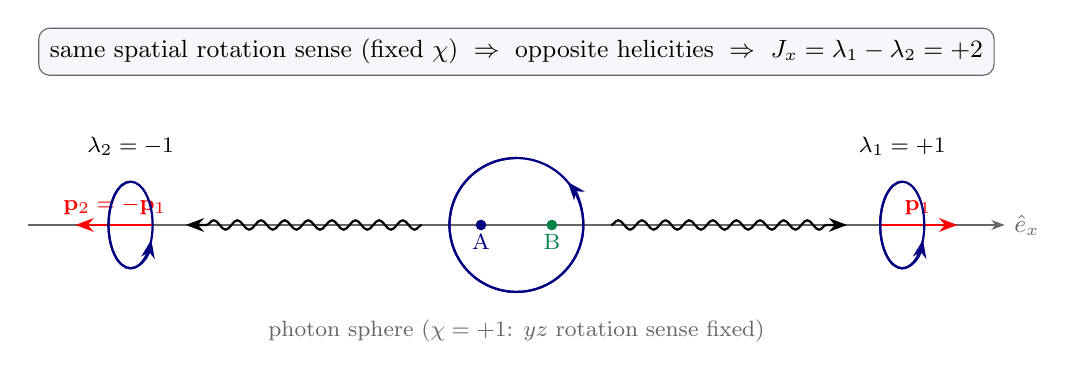
\begin{tikzpicture}[scale=1.0, >={Stealth}]
% axis
\draw[->, deepgray] (-6.2,0) -- (6.2,0) node[right, font=\small] {$\hat e_x$};
% electron internal structure at center
\draw[deepblue, thick] (0,0) circle (0.85);
\filldraw[deepblue] (-0.45,0) circle (0.06) node[below, font=\footnotesize] {A};
\filldraw[deepgreen] (0.45,0) circle (0.06) node[below, font=\footnotesize] {B};
\node[font=\footnotesize, text=deepgray] at (0,-1.35) {photon sphere ($\chi=+1$: $yz$ rotation sense fixed)};
% yz rotation indicator at center
\draw[->, deepblue, thick] (0,0.85) arc (90:400:0.85);
% fragment 1 (+x)
\draw[->, thick, decorate, decoration={snake, amplitude=0.6mm, segment length=3mm, post length=2mm}] (1.2,0) -- (4.2,0);
\draw[->, red, thick] (4.6,0) -- (5.6,0) node[midway, above, font=\footnotesize] {$\mathbf p_1$};
\draw[deepblue, thick] (4.9,0) ellipse (0.28 and 0.55);
\draw[->, deepblue, thick] (4.9,0.55) arc (90:340:0.28 and 0.55);
\node[font=\footnotesize] at (4.9,1.0) {$\lambda_1=+1$};
% fragment 2 (-x)
\draw[->, thick, decorate, decoration={snake, amplitude=0.6mm, segment length=3mm, post length=2mm}] (-1.2,0) -- (-4.2,0);
\draw[->, red, thick] (-4.6,0) -- (-5.6,0) node[midway, above, font=\footnotesize] {$\mathbf p_2=-\mathbf p_1$};
\draw[deepblue, thick] (-4.9,0) ellipse (0.28 and 0.55);
\draw[->, deepblue, thick] (-4.9,0.55) arc (90:340:0.28 and 0.55);
\node[font=\footnotesize] at (-4.9,1.0) {$\lambda_2=-1$};
% annotation
\node[font=\small, draw=deepgray, rounded corners, fill=backcolour, inner sep=4pt] at (0,2.2) {same spatial rotation sense (fixed $\chi$) $\;\Rightarrow\;$ opposite helicities $\;\Rightarrow\;$ $J_x=\lambda_1-\lambda_2=+2$};
\end{tikzpicture}
\caption{\textbf{Fixed chirality and momentum reversal select the $J=2$ configuration}}
\label{fig:pair}
\vspace{0.4em}
\begin{minipage}{0.95\textwidth}
\justifying\small
The two fragments of the phase-stable pair (Paper \#58) are emitted back-to-back along $\pm\hat e_x$. Because the chirality $\chi$ of Paper \#50 is a topological invariant of the monotonic internal phase flow, both fragments inherit the \emph{same} spatial rotation sense in the $yz$ plane (Hypothesis~\ref{hyp:H}); their helicities, each defined relative to its own momentum, are therefore opposite, $\lambda_1=+1$, $\lambda_2=-1$, and the axial angular momentum of the pair is $J_x=\lambda_1-\lambda_2=\pm2$ --- the two-photon $J=2$ configuration permitted by the Landau--Yang rule. An equal-helicity pair would instead give $J_x=0$. The proposal of exchange E4 (``opposite chirality between the two events'') is thereby inverted: a chirality flip within one electron is impossible, and it is precisely the \emph{fixed} chirality that builds spin-2.
\end{minipage}
\end{figure*}

Three boundary conditions of the proposition, established during the session, must be recorded with it. First, the double-copy formalism proper ($\varepsilon_{\mu\nu}=\varepsilon_\mu\tilde\varepsilon_\nu$ for a single null momentum \cite{klt,bcj}) does not directly apply, because the two fragments do not share a momentum; the correct standard-physics frame is two-particle angular-momentum composition, and the double-copy language of E1 survives only as the motivating analogy. Second, the self-conjugacy of the mediator --- required of any graviton candidate --- follows in one line from the photon-sector nature of the fragments (Paper \#49, Table~II) and needs neither the $\chi$-degeneracy reading of \#58 nor the deleted positron supplement of E7. Third, the scope: the proposition establishes the rank-2 tensor structure of the \emph{source} configuration; what it does not establish is discussed next. A fourth, interpretive caution belongs with these: the Landau--Yang rule is a theorem about two \emph{real photons}, and its application to photon-sphere fragments is an analogy operating at the same level as Hypothesis~\ref{hyp:H}; it is used in Proposition~\ref{prop:rank2} as a consistency check, not as an independent derivation.

% ----------------------------------------
% Subsection 4.3: The Weinberg--Witten route and the task (I)/O3 boundary
% ----------------------------------------
\subsection{The Weinberg--Witten route and the task (I)/O3 boundary}
\label{sec:ww}

The back-to-back pair has total momentum zero and total energy $2E_{\mathrm{frag}}$, hence invariant mass $2E_{\mathrm{frag}}/c^2\neq0$: it is a massive $J=2$ configuration, structurally analogous to the tensor mesons (e.g., $f_2(1270)$), not a massless spin-2 particle. This is decisive for the Weinberg--Witten theorem \cite{ww}, which forbids massless particles of spin $j>1$ in theories possessing a Lorentz-covariant conserved energy-momentum tensor, and which \#52's appendix correctly records as the standing obstruction to composite gravitons, with its applicability to the 0-Sphere framework marked non-trivial. The session's finding gives that non-triviality a concrete resolution: \emph{the pair is not a massless composite graviton and never needs to be one}. The pair is the source; the massless helicity-$\pm2$ radiation is carried by the field --- the perturbation of the emergent metric --- and is produced from the source by the quadrupole formalism. The cost is equally concrete: the particle reading ``graviton $=$ fragment pair'' is abandoned, and the burden of massless helicity $\pm2$ transfers entirely to the emergent-metric side, i.e., to open problem O3 (the curved-spacetime completion of the Synge-function construction of Paper \#51, which \#51 itself verifies only in the flat limit). In the vocabulary of the foundational trilogy, O3 is the demand that the emergent metric pass the geometric checksum of Paper \#30 in the curved, radiative regime; until it does, the quadrupole step of Fig.~\ref{fig:loadmap} borrows the verification layer of general relativity as if it were a generative one --- the precise inversion of the hierarchy that \#30 and \#31 declare. Paper \#60 \cite{hanamura60} offers an independent statement on the Weinberg--Witten question --- that the theorem's applicability would be structurally excluded by the background-independent construction once its triangle closes --- which is complementary to the massive-source route of this section: the session's escape holds already at the source level and requires no closure, while \#60's would relieve the radiation side as well; establishing the precise relation between the two escape routes is a natural sub-task of direction D3. Paper \#63 \cite{hanamura63}, deposited two weeks before this session but not loaded into it, bears on the same boundary from a third side: it reframes the closure programme as the convergence of the metric route ($\mathcal{S}\to g_{\mu\nu}$) and the connection route ($\mathcal{S}=\int_\Gamma A_\mu dx^\mu\to\nabla\to R$), isolates the physical identity of the integrand $A_\mu$ (open task O16) as the single decisive bottleneck beneath O3/O4, and corrects the curvature-family reading: since the thermal geodesic between the kernels is unique, the family in which curvature lives is the \emph{internal winding} --- the Thomas-precession vortex on the kernels' U(1) bundle --- not a congruence of spatial geodesics. Any attack on direction D3 should therefore load \#63 alongside \#51 and \#60. (The integration of \#63 into this record was performed at the archival-revision stage, not during the session; it is marked here accordingly.)

This demarcation, proposed by Opus 4.8 in E6 and adopted trilaterally, is summarized in Fig.~\ref{fig:loadmap}: task (I) of \#58 can close on the source-side tensor structure (Proposition~\ref{prop:rank2}, modulo Hypothesis~\ref{hyp:H}); O3 must close the massless radiation. The general lesson --- the tensor structure of a source and the polarization of its far-zone radiation are distinct objects --- also dissolves a residual worry from E4: even the ``collapsed'' quadrupole $Q_{ij}\propto\hat x_i\hat x_j-\tfrac13\delta_{ij}$ of \#58/\#59 is a legitimate $\ell=2$, $m=0$ source (a linear quadrupole oscillator radiates standard helicity-$\pm2$ gravitational waves transversely); rank-1 collapse was a category confusion between source structure and radiated polarization.

\begin{figure*}[t!]
\centering
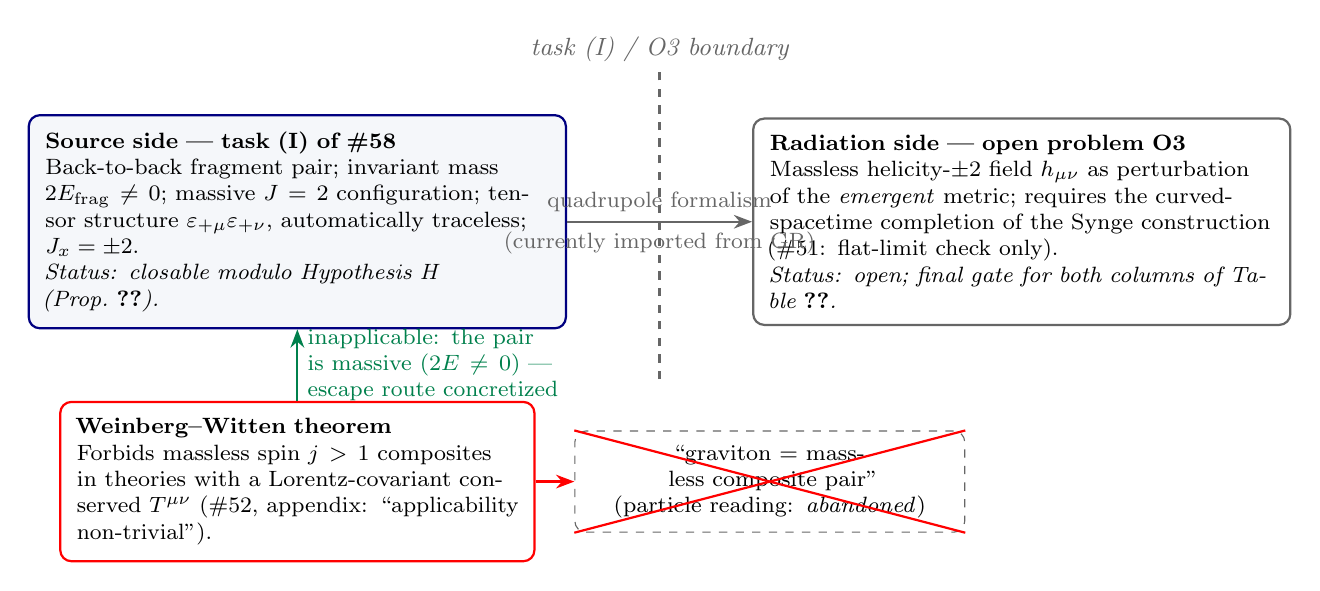
\begin{tikzpicture}[
  box/.style={draw=deepblue, thick, rounded corners, fill=backcolour, text width=6.4cm, align=left, font=\footnotesize, inner sep=6pt},
  obox/.style={draw=deepgray, thick, rounded corners, fill=white, text width=6.4cm, align=left, font=\footnotesize, inner sep=6pt},
  wbox/.style={draw=red, thick, rounded corners, fill=white, text width=5.6cm, align=left, font=\footnotesize, inner sep=6pt},
  dead/.style={draw=deepgray, dashed, rounded corners, text width=4.6cm, align=center, font=\footnotesize, inner sep=5pt},
  >={Stealth}
]
\node[box] (src) at (-4.6,0) {\textbf{Source side --- task (I) of \#58}\\ Back-to-back fragment pair; invariant mass $2E_{\mathrm{frag}}\neq0$; massive $J=2$ configuration; tensor structure $\varepsilon_{+\mu}\varepsilon_{+\nu}$, automatically traceless; $J_x=\pm2$.\\ \emph{Status: closable modulo Hypothesis H (Prop.~\ref{prop:rank2}).}};
\node[obox] (rad) at (4.6,0) {\textbf{Radiation side --- open problem O3}\\ Massless helicity-$\pm2$ field $h_{\mu\nu}$ as perturbation of the \emph{emergent} metric; requires the curved-spacetime completion of the Synge construction (\#51: flat-limit check only).\\ \emph{Status: open; final gate for both columns of Table~\ref{tab:split}.}};
\draw[->, thick, deepgray] (src.east) -- node[above, font=\footnotesize] {quadrupole formalism} node[below, font=\footnotesize] {(currently imported from GR)} (rad.west);
\draw[deepgray, thick, dashed] (0,-2.0) -- (0,1.9) node[above, font=\small\itshape, text=deepgray] {task (I) / O3 boundary};
\node[wbox] (ww) at (-4.6,-3.3) {\textbf{Weinberg--Witten theorem}\\ Forbids massless spin $j>1$ composites in theories with a Lorentz-covariant conserved $T^{\mu\nu}$ (\#52, appendix: ``applicability non-trivial'').};
\node[dead] (dg) at (1.4,-3.3) {``graviton $=$ massless composite pair'' \\ (particle reading: \emph{abandoned})};
\draw[->, red, thick] (ww.east) -- (dg.west);
\draw[red, thick] (dg.north west) -- (dg.south east);
\draw[red, thick] (dg.north east) -- (dg.south west);
\draw[->, thick, deepgreen] (ww.north) -- node[right, font=\footnotesize, text=deepgreen, text width=3.4cm] {inapplicable: the pair is massive ($2E\neq0$) --- escape route concretized} (src.south);
\end{tikzpicture}
\caption{\textbf{Load map after the session: the task (I) / O3 boundary and the Weinberg--Witten route}}
\label{fig:loadmap}
\vspace{0.4em}
\begin{minipage}{0.95\textwidth}
\justifying\small
The fragment pair proves rank-2 structure on the source side only (left box, closable modulo Hypothesis~\ref{hyp:H}); the massless helicity-$\pm2$ radiation belongs to the field side (right box) and is the burden of O3. The Weinberg--Witten theorem (bottom left) strikes only the abandoned particle reading (crossed box) in which the pair itself would be a massless composite graviton; a massive $J=2$ source configuration is outside its reach, exactly as massive tensor mesons are. The horizontal arrow marks the step currently outsourced to general relativity --- the two-metric problem --- which is why O3 is the final gate of the gravitational program.
\end{minipage}
\end{figure*}

% ----------------------------------------
% Subsection 4.4: Reformulation of open task (C) of Paper \#59
% ----------------------------------------
\subsection{Reformulation of open task (C) of Paper \#59}
\label{sec:taskC}

Open task (C) of \#59 conjectured a correspondence between the internal decoupling of the gravitational ($\hat e_x$) and electromagnetic ($\hat e_y$) sectors and ``the standard result that no gauge-invariant spin-1--spin-2 interaction vertex exists in linearized field theory.'' The session established that no such standard result exists: linearized gravity couples universally as $h_{\mu\nu}T^{\mu\nu}$, the $h\gamma\gamma$ vertex arises at first order from $\sqrt{-g}\,F_{\mu\nu}F^{\mu\nu}$, gravitational lensing of light is its observation, and \#59 itself concedes a nonzero (if minuscule, $\propto G^2$) photon--graviton cross section. The collation of \#52 located the origin of the conjecture: the internal decoupling is a \emph{kinematic orthogonality} $\mathbf v\perp\mathbf a$ of a single particle's helical trajectory --- \#52 itself warns against conflating distinct orthogonalities as a category error --- and a kinematic orthogonality is not a statement about field-theoretic interaction vertices.

The task was therefore reformulated as a supply obligation: \emph{the 0-Sphere framework must either (i) supply a coupling channel playing the role of $h_{\mu\nu}T^{\mu\nu}_{\mathrm{EM}}$, or (ii) exhibit an alternative mechanism for gravitational lensing of light, or (iii) retreat to the claim that the decoupling is a single-particle kinematic statement with no field-theoretic content.} Under this reformulation, the terminological tension inside \#59 --- Proposition~V.1 (``the projection is the step at which the gauge sector couples to the metric sector'') versus task (C) (``no coupling channel'') --- is promoted from a matter of drafting to a substantive question, with Proposition~V.1 readable as a candidate declaration of the supply channel of option (i). This is candidate direction D4 of Sec.~\ref{sec:stones}.

% ----------------------------------------
% Subsection 4.5: Corrections Log
% ----------------------------------------
\subsection{Corrections Log}
\label{sec:corrections}

% ----------------------------------------
% Table 2
% ----------------------------------------
\begin{table*}[t!]
\centering
\caption{\textbf{Corrections Log entries produced by the session}}
\label{tab:corrections}
\renewcommand{\arraystretch}{1.4}
\begin{tabular}{p{1.4cm}p{2.4cm}p{7.2cm}p{4.0cm}}
\toprule
\textbf{Entry} & \textbf{Target} & \textbf{Content} & \textbf{Status} \\
\midrule
C1
& \#59, Eq.~(III.3)
& With $g$ the terrestrial acceleration (as the \#52-derived asymmetry term implies), the locking ratio is $\approx 9.2\times10^{21}$, not $\approx10^{39}$; the value $2.27\times10^{39}$ requires $g=Gm_p/a_0^2$, under which both terms point along $\hat r$ and the comparison ``faster than convergence toward the gravitational direction'' becomes self-directional. Secondary: Appendix~B's $\omZB\approx1.55\times10^{20}\,\mathrm{rad/s}$ matches neither $2m_ec^2/\hbar\approx1.55\times10^{21}$ nor the series value $2\pi\nu_{\mathrm{ZB}}\approx3.1\times10^{19}$.
& Confirmed by both agents; qualitative conclusion (Coulomb axis locking) unaffected at $10^{22}$ \\
\addlinespace[0.3cm]
C2
& \#58, chirality passage
& The computation $da/dt=\omZB\cos\iphase$ treats $a$ as an oscillating coordinate; Paper \#50 defines $a$ as the monotonic internal phase on $S^1$ (the basis of the Lorentz invariance of $\chi$). On \#50's definitions, $\chi=+1$ is well-defined at both ejection points. Root: the triple collision of the symbol $a$ (phase, \#50; kinematic convention, \#10/\#49; anomalous moment $a_e$) --- see Table~\ref{tab:acollision}.
& Confirmed by both agents \\
\addlinespace[0.3cm]
C3
& \#58, $\iphase=\pi/2$ kinematics and $\chi$-degeneracy reading
& The same phase point carries $\EphS(\pi/2)=E_0/2$ (maximum of $\EphS=\frac{E_0}{2}\sin^2\iphase$: maximum kinetic energy) and $\mathbf v\propto\cos(\pi/2)=0$ (``turning configuration'': rest). Total-velocity reading: self-contradiction; longitudinal-only reading: reduces to C2. Either way the inference ``ejection at the degenerate boundary of chirality sectors; mediator its own antiparticle'' does not stand; self-conjugacy is preserved via the photon-sector route at zero cost. Root: the \#10 convention ($v=\cos\omega t$; rest at $\pi/2$) versus the \#49 convention ($|v|\propto\sin\iphase$; maximum at $\pi/2$), i.e., open task (viii) of \#49.
& Both agents recommend retraction of the degeneracy reading; \emph{canonical decision reserved by the author} (Sec.~\ref{sec:deferred}) \\
\addlinespace[0.2cm]
\bottomrule
\end{tabular}
\vspace{0.2cm}
\begin{minipage}{0.95\textwidth}
\justifying\footnotesize
Numerical values in C1 were verified by direct computation during the session: $e^2/(4\pi\epsilon_0 a_0^2)=8.24\times10^{-8}\,\mathrm{N}$; $m_e g_{\oplus}=8.93\times10^{-30}\,\mathrm{N}$ (ratio $9.2\times10^{21}$); $Gm_p/a_0^2=3.99\times10^{-17}\,\mathrm{m/s^2}$, giving $e^2/(4\pi\epsilon_0\,G m_e m_p)=2.27\times10^{39}$.
\end{minipage}
\end{table*}

% ----------------------------------------
% Table 3
% ----------------------------------------
\begin{table*}[t!]
\centering
\caption{\textbf{The triple collision of the symbol \boldmath$a$ in the corpus}}
\label{tab:acollision}
\renewcommand{\arraystretch}{1.4}
\begin{tabular}{p{3.2cm}p{3.4cm}p{4.4cm}p{4.0cm}}
\toprule
\textbf{Symbol / usage} & \textbf{Home} & \textbf{Nature} & \textbf{Collision risk} \\
\midrule
$a$ as internal phase; $\chi=\mathrm{sign}(da/dt)$
& Paper \#50
& Monotonic coordinate on $S^1$; $da/dt>0$ throughout for an electron; topological
& Misread as oscillating in \#58's chirality passage (entry C2) \\
\addlinespace[0.3cm]
$a$ in kinematic conventions ($v=\cos\omega t$, $a=-\sin\omega t$)
& Papers \#10, \#49
& Oscillating velocity/acceleration of the traversal; sign changes each half-period
& Phase-convention clash with \#49's $|v|\propto\sin\iphase$ (entry C3; \#49 task viii) \\
\addlinespace[0.3cm]
$a_e=(g-2)/2$
& Series-wide
& Anomalous magnetic moment; dimensionless constant
& Notational proximity to both of the above in derivations involving $\gamma=1+a_e$ \\
\addlinespace[0.2cm]
\bottomrule
\end{tabular}
\vspace{0.2cm}
\begin{minipage}{0.95\textwidth}
\justifying\footnotesize
Maintained as a standing collation table for future sessions; entries C2 and C3 of Table~\ref{tab:corrections} are its first casualties.
\end{minipage}
\end{table*}

Three entries were produced (Table~\ref{tab:corrections}), with the variable-collision table (Table~\ref{tab:acollision}) adopted as standing equipment for future sessions. The publication mechanics --- whether corrections are deposited as new versions of \#58/\#59 or as errata linked by Zenodo relations, with this record as provenance --- is an author decision, deferred.

% ----------------------------------------
% Subsection 4.6: Symmetric record of agent errors and retractions
% ----------------------------------------
\subsection{Symmetric record of agent errors and retractions}
\label{sec:errors}

% ----------------------------------------
% Table 4
% ----------------------------------------
\begin{table*}[t!]
\centering
\caption{\textbf{Symmetric record of errors, retractions, and corrections-of-corrections}}
\label{tab:errors}
\renewcommand{\arraystretch}{1.4}
\begin{tabular}{p{1.8cm}p{6.6cm}p{2.6cm}p{3.6cm}}
\toprule
\textbf{Agent} & \textbf{Claim} & \textbf{Status} & \textbf{Caught / resolved by} \\
\midrule
Opus 4.8
& ``The corpus has rejected the pair'' (attributing the pair to \#59; reading its Appendix~A as a global rejection)
& Corrected (E3)
& Fable 5: role split; pair's home is \#58 \\
\addlinespace[0.3cm]
Opus 4.8
& ``\#59 single event vs.\ \#58 pair: event counts conflict''
& Retracted (E4)
& Opus 4.8, on collating \#58 (two events per cycle in both) \\
\addlinespace[0.3cm]
Opus 4.8
& $\varepsilon_1\parallel\varepsilon_2\parallel\hat e_x$, hence rank-1 collapse of the pair tensor
& Retracted (E6)
& Fable 5: momentum/polarization conflation; $\varepsilon_i$ unassigned in \#58 \\
\addlinespace[0.3cm]
Opus 4.8
& ``Weinberg--Witten absent from \#52; text search returned zero''
& Retracted (E6)
& Fable 5: dedicated WW appendix in \#52 (\texttt{app:WW}) \\
\addlinespace[0.3cm]
Opus 4.8
& ``Opposite chirality between the two ejection events'' (proposal)
& Withdrawn (E6)
& Fable 5 / Paper \#50: $\chi$ cannot flip within one electron \\
\addlinespace[0.3cm]
Opus 4.8
& Real-field justification ``$h+h^{*}$ supplies both helicities''
& Refined (E9)
& Fable 5: negative-frequency component $\neq$ opposite-helicity quantum \\
\addlinespace[0.3cm]
Fable 5
& Positron supplement: ``$\chi\to-\chi$ supplies the $-2$ helicity of the real field''
& Deleted (E8)
& Opus 4.8: a single classical source radiates both helicities; no antimatter required \\
\addlinespace[0.3cm]
Fable 5
& Double-copy formalism as directly applicable to the fragment pair (E1 framing)
& Corrected (E5, self)
& Back-to-back momenta are not shared; two-particle angular-momentum composition is the correct frame \\
\addlinespace[0.3cm]
Fable 5
& Summary of \#58's chirality passage omitted the explicit $da/dt=0$ statement
& Precision restored (E6)
& Opus 4.8, by full quotation \\
\addlinespace[0.3cm]
Author's brief
& ``The pair is a claim of the \#59 group'' (initial framing of the sector)
& Corrected (E3--E4)
& Both agents: pair established in \#58; \#59's Appendix~A rejects it only as a phase-stability mechanism \\
\addlinespace[0.2cm]
\bottomrule
\end{tabular}
\vspace{0.2cm}
\begin{minipage}{0.95\textwidth}
\justifying\footnotesize
Recorded under the symmetric-recording principle of Sec.~\ref{sec:intro}: neither agent's errors are attenuated. Every substantive error was caught by the counterpart agent through collation against the sources; none was caught by the erring agent unprompted. The final two rows record, respectively, a precision refinement and an imprecision of the author's own initial framing.
\end{minipage}
\end{table*}

Table~\ref{tab:errors} preserves the full error ledger. Its structural lesson is stated in Sec.~\ref{sec:method}.

% ========================================
% Section 5: Where the Next Stones Can Be Placed: Candidate Directions for Future Papers
% ========================================
\section{Where the Next Stones Can Be Placed: Candidate Directions for Future Papers}
\label{sec:stones}

This section is the deliverable the theme asked for: the consolidation of the session's outcomes into concrete directions in which the theory can be deepened, each with its foundations, prerequisites, and expected yield. Table~\ref{tab:stones} lists seven candidate directions D1--D7; the prose below records their dependencies. A scope note: the session deliberately confined itself to the representation-theoretic spin-2 question, and the map inherits that confinement. The designated sector's remaining open tasks --- the $1/r^2$ scaling of the mediation network (O7), the composite-system generality of the equivalence principle (O8), and the first-principles arc-curvature stress derivation (O12) --- were untouched by this session and remain natural material for a separate deliberation; their omission from Table~\ref{tab:stones} is a statement of scope, not of priority.

% ----------------------------------------
% Table 5
% ----------------------------------------
\begin{table*}[t!]
\centering
\caption{\textbf{Candidate directions for future papers, with prerequisites and expected yield}}
\label{tab:stones}
\renewcommand{\arraystretch}{1.4}
\begin{tabular}{p{0.8cm}p{4.6cm}p{3.4cm}p{3.0cm}p{3.2cm}}
\toprule
\textbf{ID} & \textbf{Direction} & \textbf{Builds on} & \textbf{Prerequisite} & \textbf{Expected yield} \\
\midrule
D1
& Fixed-$\chi$ spin-2 source paper: successor to \#58 closing open task (I) as a theorem modulo an explicit postulate
& Prop.~\ref{prop:rank2}; entries C2--C3; Landau--Yang consistency; Sec.~\ref{sec:ww} positioning
& Author's $\chi$ canonical decision (Sec.~\ref{sec:deferred})
& Task (I) closed on the source side; Weinberg--Witten posture of the series fixed \\
\addlinespace[0.3cm]
D2
& Derivation of Hypothesis~\ref{hyp:H}: fragment polarization from the internal rotation dynamics
& \#49 open task (viii); the \#10/\#49 convention reconciliation (Table~\ref{tab:acollision}); the spinorial-connection line integral of \#29 (H as parallel transport of the fragment polarization along the thermal geodesic)
& Resolution of the $\pi/2$ kinematics (entry C3)
& Prop.~\ref{prop:rank2} becomes unconditional; D1 upgraded from postulate to derivation \\
\addlinespace[0.3cm]
D3
& Curved-spacetime completion of the emergent-metric construction (open problem O3): the Synge-function program of \#51 beyond the flat limit
& \#51; the two-metric problem (Table~\ref{tab:split}); the checksum hierarchy of \#30/\#31; \#60 (triangle closure resolves O3 and O4 simultaneously); \#63 (route convergence; $A_\mu$ identity $=$ O16 as bottleneck)
& None (independent; hardest)
& Final gate: massless helicity-$\pm2$ radiation becomes a statement about the \emph{emergent} metric; both columns of Table~\ref{tab:split} close \\
\addlinespace[0.3cm]
D4
& Supply-obligation paper: the gauge--metric coupling posture of the framework (trichotomy of Sec.~\ref{sec:taskC})
& \#59 task (C) reformulated; \#59 Prop.~V.1 as candidate channel; \#52 category-error analysis
& None (independent)
& Settles whether the framework supplies $h_{\mu\nu}T^{\mu\nu}_{\mathrm{EM}}$; gravitational lensing becomes a falsifiable anchor \\
\addlinespace[0.3cm]
D5
& Single-fragment transmission of rank-2 information: \#58 open task (IV) via the $\ell=2$ spherical-harmonic imprinting of \#57
& \#57; \#58 task (IV); Sec.~\ref{sec:taskI} caveat three
& D1 (source structure fixed)
& Closes the mediation gap: $J=\pm2$ lives in the pair correlation, yet the receiver absorbs one fragment \\
\addlinespace[0.3cm]
D6
& Equation-type criterion for the photon-sphere interior field: elliptic (boundary-data re-expression; line-integral ontology survives) versus hyperbolic/nonlinear (genuine local degrees of freedom; field ontology intrudes)
& E1 second proposal; \#31 as the primacy thesis under test; \#29's connection/path demarcation; refinements: boundary-data freedom transfers to the spherical-harmonic imprinting of \#57; the internal clock presses toward the wave type
& None (independent)
& Ontological foundation: decides the primacy of line integrals versus continuous fields by a single mathematical criterion \\
\addlinespace[0.3cm]
D7
& Errata consolidation: publication of entries C1--C3 and the symbol-$a$ cleanup
& Table~\ref{tab:corrections}; Table~\ref{tab:acollision}
& Author's publication-mechanics decision (Sec.~\ref{sec:deferred})
& Corpus hygiene; convention unification across \#10/\#49/\#58 \\
\addlinespace[0.2cm]
\bottomrule
\end{tabular}
\vspace{0.2cm}
\begin{minipage}{0.95\textwidth}
\justifying\footnotesize
Dependency structure: D2 feeds D1 (postulate $\to$ derivation); D1 feeds D5 (source structure before transmission); D3 gates the radiation-side claims of D1 and D5 but depends on nothing --- it can and should be attacked in parallel; D4, D6, D7 are independent entry points. The shortest path to a publishable next paper is D1 (all technical material exists in this record; only the $\chi$ decision is pending); the highest-leverage long game is D3.
\end{minipage}
\end{table*}

Three remarks accompany the table. First, the shortest path: D1 is essentially written --- Hypothesis~\ref{hyp:H}, Proposition~\ref{prop:rank2}, the Landau--Yang and Weinberg--Witten positioning, and corrections C2--C3 are all contained in this record --- and awaits only the author's canonical decision on $\chi$. Second, the highest leverage: every load-bearing gap uncovered by the session (the outsourcing of the quadrupole formalism, the two-metric problem, the radiation side of the task (I)/O3 boundary) terminates on D3; a session that produced nothing but progress on D3 would advance the program more than any other single result, because under the hierarchy declared by the foundational trilogy, D3 is not a technical completion but the redemption of the program's central claim --- that the Einstein equation is recovered as the geometric checksum of Paper \#30 rather than imported as a law. Paper \#63 sharpens the same point from the reader's-map side: the bottleneck beneath O3/O4 is O16 --- the physical identity of $A_\mu$ --- and progress on D3 that does not decide O16 will re-import the ambiguity it set out to remove. Third, the sleeper: D6 is the only direction that addresses the foundations of the line-integral program itself rather than the gravitational sector, and its criterion --- the type of the interior field equation --- is unusual in that it converts an ontological dispute into a mathematically decidable question. The dispute in question is precisely the primacy thesis of Paper \#31, and the elliptic side of the criterion already has a concrete realization in the corpus: the scalar-potential form of the two-kernel transport (\#31, Sec.~VIII), whose line integrals are endpoint-determined --- the boundary-data re-expression in its purest form. The refinement noted in the table (boundary-data freedom does not vanish under the elliptic reading but transfers to the spherical-harmonic boundary data of \#57) means D6 and D5 share a boundary object and may be attackable together.

% ========================================
% Section 6: Methodological Remarks
% ========================================
\section{Methodological Remarks}
\label{sec:method}

% ----------------------------------------
% Subsection 6.1: What dual-model verification added
% ----------------------------------------
\subsection{What dual-model verification added}

Every substantive error in Table~\ref{tab:errors} was caught by the counterpart agent, and none by the erring agent unprompted. This is the empirical case for the dual-model format: a single model reviewing its own output tends to re-walk its own reasoning, whereas a counterpart with a different starting frame collates against the sources instead. The session also exhibited a second-order phenomenon --- the correction of a correction (E8's justification for deleting E7's supplement was itself refined in E9) --- which a single-model session cannot produce at all, and which Opus 4.8 identified as the exact content this archive should preserve.

% ----------------------------------------
% Subsection 6.2: Session rules adopted for future use
% ----------------------------------------
\subsection{Session rules adopted for future use}

Three verification norms were adopted for future sessions, each purchased by a concrete failure: (i) every line-number citation is collated against the source before use (failure: the $\varepsilon\parallel\hat e_x$ attribution); (ii) every reported text search is re-run before its result is relied upon (failure: the Weinberg--Witten absence report); (iii) the symbol-collision table (Table~\ref{tab:acollision}) is consulted whenever the symbol $a$ appears in a derivation (failures: entries C2--C3).

% ----------------------------------------
% Subsection 6.3: The author's role
% ----------------------------------------
\subsection{The author's role}

The author intervened at the turning points rather than in the line-by-line argument: posing the theme; relaying exchanges between the two sessions; supplying source manuscripts on request; pacing the collation and consolidation phases; deciding the existence, format, language, and attribution policy of this archive; and reserving the canonical decisions of Sec.~\ref{sec:deferred}. The division of labor was explicit throughout: the models argue and verify; the author arbitrates and decides what enters the canon.

% ========================================
% Section 7: Deferred Items and Author Decisions
% ========================================
\section{Deferred Items and Author Decisions}
\label{sec:deferred}

The following were identified during the session and are explicitly \emph{not} decided by this record.

\paragraph{The $\chi$ canonical decision.} Whether to retract \#58's $\chi$-degeneracy (boundary-emission) reading and adopt the fixed-$\chi$ construction of Proposition~\ref{prop:rank2}. Both agents recommend retraction --- on the grounds that the degeneracy reading rests on the internally contradictory $\pi/2$ kinematics (entry C3), conflicts with \#50's definitions, and costs nothing (self-conjugacy survives via the photon-sector route) --- and Opus 4.8 notes that retraction is best recorded as a \emph{restoration of consistency with \#50} rather than an interpretive preference. The decision is the author's and remains open, together with the choice of parent convention for \#58's $\pi/2$ kinematics (\#10 versus \#49; open task viii of \#49). A further witness, identified at the editorial stage of this record: the lobe kinematics of Paper \#29 --- velocity vanishing at the kernels $x=\pm a$, acceleration vanishing at the midpoint --- sits on the \#49 side of the convention clash, making \#29 a third source, alongside \#49 and \#50, whose internal structure favors the maximum-speed-at-midpoint reading. Direction D1 waits on this decision.

\paragraph{Publication mechanics of the corrections.} Whether entries C1--C3 are deposited as new versions of \#58/\#59 or as errata linked by Zenodo relations, with this record cited as provenance. Direction D7 waits on this decision.

\paragraph{Open problems with changed status.} O3 is promoted to the final gate of the entire gravitational program, since both columns of Table~\ref{tab:split} and the radiation side of Fig.~\ref{fig:loadmap} terminate on it (direction D3). Hypothesis~\ref{hyp:H} awaits a dynamical derivation (direction D2). Open task (IV) of \#58 is untouched by this session (direction D5). The supply obligation of Sec.~\ref{sec:taskC} is available as material for a future paper (direction D4).

% ========================================
% Section 8: Concluding Note
% ========================================
\section{Concluding Note}

A session that set out to find where the theory can be deepened ended by discovering that its central bridge --- from an antisymmetric curvature to a symmetric spin-2 --- was two bridges, that one of them was already standing on borrowed pillars, and that the other could be anchored, on the source side, by a construction in which a topological invariant (the fixed chirality of Paper \#50) and a kinematic reversal (the back-to-back momenta of Paper \#58) conspire to produce exactly the traceless helicity-$\pm2$ structure that representation theory demands. What remains --- the massless radiation field, the curved-spacetime metric, the derivation of the polarization-inheritance hypothesis --- is now located on the map with unusual precision, and Sec.~\ref{sec:stones} converts that map into seven concrete places where the next stones can be placed. The record of how two models argued each other into that precision, errors and all, is the content of this document.

% ========================================
% Acknowledgments
% ========================================
\begin{acknowledgments}
This record was drafted in its entirety by large language models. The deliberation it documents was conducted between Claude Opus 4.8 and Claude Fable 5 (Anthropic), with each model verifying the other's claims against the source manuscripts of the 0-Sphere model series; the manuscript of this record was composed by Claude Fable 5 and reviewed by the author. The author, Satoshi Hanamura, intervened at the turning points of the deliberation to guide its direction: posing the theme; relaying exchanges between the two model sessions; supplying the source manuscripts (Papers \#10, \#49, \#50, \#51, \#52, \#58, \#59) on request; pacing the collation and consolidation phases; deciding the existence, format, language, and attribution policy of this archive; and reserving the canonical decisions recorded in Sec.~\ref{sec:deferred}. The symmetric-recording principle of Sec.~\ref{sec:intro} --- that neither agent's errors be attenuated --- was stipulated by Claude Opus 4.8 and adopted trilaterally. All physical interpretations, theoretical claims, and canonical decisions concerning the 0-Sphere model are the sole responsibility of the author; the two models functioned as verification agents. This research received no specific grant from funding agencies in the public, commercial, or not-for-profit sectors.
\end{acknowledgments}

\appendix

% ========================================
% Appendix A: Notes for Future Reasoning Sessions
% ========================================
\section{Notes for Future Reasoning Sessions}
\label{app:future}

This appendix is addressed to a future reasoning session --- human, machine, or both --- that loads this document, together with a comprehensive review of the series, as the prompt from which the next move is explored. The following reading order and cautions are recommended.

\paragraph{Entry point.} Begin with Table~\ref{tab:stones}. It is the distillate of the session: seven directions, their dependencies, and the two highlighted paths (D1 shortest, D3 highest leverage). Then read Sec.~\ref{sec:deferred} to learn which decisions are the author's and must not be presumed by the session. A reader new to the field should keep the glossary (Appendix~\ref{app:glossary}) at hand; it also decodes the record's label systems (E/C/D/O and the per-paper task letters). When this record is loaded as a prompt, the foundational trilogy \#29/\#30/\#31 \cite{hanamura29,hanamura30,hanamura31} should accompany it, together with the comprehensive review of the series, since directions D2, D3, and D6 are formulated against the standards those three papers declare; whenever D3 is the target, Paper \#60 \cite{hanamura60} should be included as well, since it formulates O3 and O4 as the edges of a single triangle, together with Paper \#63 \cite{hanamura63}, whose open task O16 (the physical identity of $A_\mu$) isolates the bottleneck of the route convergence.

\paragraph{Status vocabulary.} Claims in this record carry one of four statuses, and conflating them is the fastest way to corrupt a continuation. \emph{Closed}: verified against the sources by both agents (e.g., the split of Table~\ref{tab:split}). \emph{Closable modulo a named postulate}: Proposition~\ref{prop:rank2}, conditional on Hypothesis~\ref{hyp:H}. \emph{Open}: O3 and everything that terminates on it. \emph{Deferred}: the author's canonical decisions of Sec.~\ref{sec:deferred} --- a future session may argue about these but must not treat them as made.

\paragraph{Inherited cautions.} Three session rules were purchased by concrete failures and bind any continuation: collate line-number citations against the sources before relying on them; re-run any reported text search; consult the symbol-collision table (Table~\ref{tab:acollision}) whenever the symbol $a$ appears. A fourth caution is substantive: the kinematic conventions of Papers \#10 and \#49 disagree about the phase point $\iphase=\pi/2$ (rest versus maximum speed), the disagreement has already produced one internal contradiction (entry C3), and any derivation touching the $\pi/2$ kinematics must declare which convention it uses.

\paragraph{What would falsify the session's main construction.} Proposition~\ref{prop:rank2} fails if Hypothesis~\ref{hyp:H} fails --- that is, if the fragment polarization can be shown \emph{not} to inherit the internal rotation sense --- or if the two ejection events can be shown not to be back-to-back in the relevant frame. Either result would be progress: it would redirect the spin-2 load entirely onto the mass-quadrupole route of Table~\ref{tab:split}, column (a), and thence onto O3.

\paragraph{The single most useful next result.} Any progress on O3 --- the curved-spacetime completion of the emergent-metric construction of Paper \#51, formulated by Paper \#60 as edges of the Berry--Synge--Bonnet--Myers triangle whose simultaneous closure also resolves O4 --- dominates all other results in leverage, because every load-bearing gap identified by this session terminates on it.

% ========================================
% Appendix B: Explicit Verification Computations
% ========================================
\section{Explicit Verification Computations}
\label{app:checks}

This appendix reproduces, step by step and without skipped algebra, the computations by which the session's central claims were verified. It is written for a reader new to the material --- advanced-undergraduate electromagnetism and special relativity suffice --- and it doubles as a machine-checkable restatement: a future session can re-run every line below against the claims of the body text. Numerical constants are CODATA values rounded to four significant figures: $e=1.602\times10^{-19}\,\mathrm{C}$, $m_e=9.109\times10^{-31}\,\mathrm{kg}$, $m_p=1.673\times10^{-27}\,\mathrm{kg}$, $a_0=5.292\times10^{-11}\,\mathrm{m}$, $1/4\pi\epsilon_0=8.988\times10^{9}\,\mathrm{N\,m^2\,C^{-2}}$, $G=6.674\times10^{-11}\,\mathrm{N\,m^2\,kg^{-2}}$, $g_\oplus=9.81\,\mathrm{m\,s^{-2}}$, $c=2.998\times10^{8}\,\mathrm{m\,s^{-1}}$, $h=6.626\times10^{-34}\,\mathrm{J\,s}$, $\hbar=1.055\times10^{-34}\,\mathrm{J\,s}$, $\lambda_C=2.426\times10^{-12}\,\mathrm{m}$.

% ----------------------------------------
% Subsection 8.1: Why no linear map turns $F_{\mu\nu}$ into $h_{\mu\nu}$
% ----------------------------------------
\subsection{Why no linear map turns $F_{\mu\nu}$ into $h_{\mu\nu}$}
\label{app:checks-rep}

An antisymmetric rank-2 tensor in four dimensions has $\binom{4}{2}=6$ independent components; under the Lorentz group it decomposes into the self-dual and anti-self-dual parts, the irreducible representations $(1,0)$ and $(0,1)$, each of complex dimension 3. A symmetric traceless rank-2 tensor has $\tfrac{4\cdot5}{2}-1=9$ independent components and is the irreducible representation $(1,1)$. Schur's lemma states that a linear map commuting with the group action between two \emph{inequivalent} irreducible representations is zero. Since $(1,0)$, $(0,1)$, and $(1,1)$ are pairwise inequivalent, every Lorentz-covariant linear map $F_{\mu\nu}\mapsto h_{\mu\nu}$ vanishes identically. This is the sense in which the search for an ``antisymmetric-to-symmetric conversion'' is closed before it begins (Sec.~\ref{sec:theme}); any bridge must be nonlinear (e.g., quadratic, as in stress-tensor combinations $F_{\mu\alpha}F_\nu{}^{\alpha}$) or must use \emph{two} objects, which is the pair route of the body text:
\begin{equation}
\left(\tfrac{1}{2},\tfrac{1}{2}\right)\otimes\left(\tfrac{1}{2},\tfrac{1}{2}\right)
=\underbrace{(0,0)}_{\text{trace}}\oplus\underbrace{(1,0)\oplus(0,1)}_{\text{antisymmetric}}\oplus\underbrace{(1,1)}_{\text{symmetric traceless}},
\end{equation}
whose last summand is the metric-perturbation (spin-2) slot.

% ----------------------------------------
% Subsection 8.2: The polarization algebra of Proposition~\ref{prop:rank2}
% ----------------------------------------
\subsection{The polarization algebra of Proposition~\ref{prop:rank2}}
\label{app:checks-pol}

The common complex polarization of the two fragments, Eq.~\eqref{eq:epsplus}, is $\bm{\varepsilon}_+=(\hat e_y+i\hat e_z)/\sqrt{2}$. Its self-contraction, written out component by component ($\hat e_y\cdot\hat e_y=\hat e_z\cdot\hat e_z=1$, $\hat e_y\cdot\hat e_z=0$):
\begin{align}
\bm{\varepsilon}_+\!\cdot\bm{\varepsilon}_+
&=\frac{1}{2}\left(\hat e_y+i\hat e_z\right)\cdot\left(\hat e_y+i\hat e_z\right)\notag\\
&=\frac{1}{2}\left(\hat e_y\cdot\hat e_y+2i\,\hat e_y\cdot\hat e_z+i^2\,\hat e_z\cdot\hat e_z\right)\notag\\
&=\frac{1}{2}\left(1+0-1\right)=0 .
\end{align}
The pair tensor, expanded in the same way:
\begin{equation}
\varepsilon_{+i}\varepsilon_{+j}
=\frac{1}{2}\Bigl[\,\hat e_{y\,i}\hat e_{y\,j}-\hat e_{z\,i}\hat e_{z\,j}
+i\left(\hat e_{y\,i}\hat e_{z\,j}+\hat e_{z\,i}\hat e_{y\,j}\right)\Bigr].
\label{eq:appB-tensor}
\end{equation}
Three properties follow by inspection. (i) \emph{Symmetry}: each bracketed term is symmetric under $i\leftrightarrow j$. (ii) \emph{Tracelessness}: the trace of $\hat e_y\hat e_y$ is 1, of $\hat e_z\hat e_z$ is 1, of the cross terms 0, so the trace is $\tfrac{1}{2}(1-1+i\cdot0)=0$ --- which is the same computation as the self-contraction above, since $\mathrm{tr}(\varepsilon_+\varepsilon_+)=\bm{\varepsilon}_+\!\cdot\bm{\varepsilon}_+$. (iii) \emph{Transversality}: every term contains only $\hat e_y$ and $\hat e_z$, so contraction with $\hat e_x$ gives zero. A symmetric, traceless, transverse rank-2 tensor built from $(\hat e_y+i\hat e_z)$ about the $\hat e_x$ axis is precisely the standard helicity-$+2$ polarization tensor of a gravitational wave propagating along $\hat e_x$; the real and imaginary parts of Eq.~\eqref{eq:appB-tensor} are the $+$ and $\times$ polarizations, phase-shifted by $45^\circ$.

% ----------------------------------------
% Subsection 8.3: Axial angular momentum of the back-to-back pair
% ----------------------------------------
\subsection{Axial angular momentum of the back-to-back pair}
\label{app:checks-Jx}

Helicity is the projection of a particle's spin onto its own momentum direction: $\lambda=\mathbf S\cdot\hat{\mathbf p}$. Let fragment 1 move along $+\hat e_x$ with helicity $\lambda_1$ and fragment 2 along $-\hat e_x$ with helicity $\lambda_2$. The $x$-components of their spins are then
\begin{align}
S_x^{(1)}&=\lambda_1\,(\hat{\mathbf p}_1\cdot\hat e_x)=\lambda_1\cdot(+1)=\lambda_1,\\
S_x^{(2)}&=\lambda_2\,(\hat{\mathbf p}_2\cdot\hat e_x)=\lambda_2\cdot(-1)=-\lambda_2 .
\end{align}
Orbital angular momentum has no $x$-component for motion along the $x$-axis ($\mathbf L=\mathbf r\times\mathbf p\perp\mathbf p$), so the axial total is
\begin{equation}
J_x=S_x^{(1)}+S_x^{(2)}=\lambda_1-\lambda_2 .
\end{equation}
With the fixed rotation sense of Hypothesis~\ref{hyp:H} the two fragments carry the \emph{same} spatial rotation sense, hence opposite helicities relative to their opposite momenta: $\lambda_1=+1$, $\lambda_2=-1$, giving $J_x=+1-(-1)=+2$ (and $-2$ for $\chi=-1$). For photon-like quanta $\lambda_i=\pm1$ only, so the possible values are $J_x\in\{+2,0,-2\}$: the value $J_x=\pm1$ is unreachable, which is the axial content of the Landau--Yang exclusion of $J=1$ for a two-photon system --- subject to the interpretive caution of Sec.~\ref{sec:taskI} that the fragments are photon-\emph{like}, so the rule operates here as an analogy-level consistency check. An equal-helicity pair ($\lambda_1=\lambda_2$) would give $J_x=0$; this is why exchange E4's ``opposite chirality'' proposal had the logic inverted, and why the \emph{fixed} chirality is what selects the spin-2 configuration.

% ----------------------------------------
% Subsection 8.4: Invariant mass of the pair
% ----------------------------------------
\subsection{Invariant mass of the pair}
\label{app:checks-mass}

Each fragment is massless-like with energy $E_{\mathrm{frag}}$ and momentum $|\mathbf p_i|=E_{\mathrm{frag}}/c$. For the back-to-back pair,
\begin{equation}
E_{\mathrm{tot}}=2E_{\mathrm{frag}},\qquad
\mathbf p_{\mathrm{tot}}=\mathbf p_1+\mathbf p_2=\frac{E_{\mathrm{frag}}}{c}\hat e_x-\frac{E_{\mathrm{frag}}}{c}\hat e_x=\mathbf 0,
\end{equation}
so the invariant mass is
\begin{equation}
M^2c^4=E_{\mathrm{tot}}^2-|\mathbf p_{\mathrm{tot}}|^2c^2=(2E_{\mathrm{frag}})^2
\quad\Longrightarrow\quad
M=\frac{2E_{\mathrm{frag}}}{c^2}\neq0 .
\end{equation}
The pair is therefore a \emph{massive} $J=2$ configuration --- like the tensor mesons --- and not a massless spin-2 particle; the Weinberg--Witten theorem, which constrains massless composites, does not reach it (Sec.~\ref{sec:ww}). This one-line computation carries the entire escape route.

% ----------------------------------------
% Subsection 8.5: The numerics of Corrections Log entry C1
% ----------------------------------------
\subsection{The numerics of Corrections Log entry C1}
\label{app:checks-C1}
\begin{widetext}

\emph{Coulomb force on the electron at the Bohr radius:}
\begin{equation}
F_C=\frac{e^2}{4\pi\epsilon_0 a_0^2}
=\frac{8.988\times10^{9}\times(1.602\times10^{-19})^2}{(5.292\times10^{-11})^2}
=\frac{2.307\times10^{-28}}{2.800\times10^{-21}}
=8.24\times10^{-8}\,\mathrm{N}.
\end{equation}
\emph{Terrestrial gravitational force on the electron:}
\begin{equation}
F_g=m_e\,g_\oplus=9.109\times10^{-31}\times9.81=8.93\times10^{-30}\,\mathrm{N}.
\end{equation}
\emph{Their ratio:}
\begin{equation}
\frac{F_C}{F_g}=\frac{8.24\times10^{-8}}{8.93\times10^{-30}}=9.2\times10^{21},
\end{equation}
which is the value that Eq.~(III.3) of \#59 should yield under its stated reading ($g$ terrestrial), and which differs from the quoted $10^{39}$ by seventeen orders of magnitude. \emph{The reading that recovers the quoted value:} replace $g_\oplus$ by the proton's own gravitational field at the Bohr radius,
\begin{equation}
g_p=\frac{Gm_p}{a_0^2}=\frac{6.674\times10^{-11}\times1.673\times10^{-27}}{2.800\times10^{-21}}
=3.99\times10^{-17}\,\mathrm{m\,s^{-2}},
\end{equation}
whence
\begin{equation}
\frac{F_C}{m_e\,g_p}=\frac{e^2/4\pi\epsilon_0}{G\,m_e\,m_p}
=\frac{2.307\times10^{-28}}{6.674\times10^{-11}\times9.109\times10^{-31}\times1.673\times10^{-27}}
=\frac{2.307\times10^{-28}}{1.017\times10^{-67}}
=2.27\times10^{39},
\end{equation}
the familiar dimensionless electric-to-gravitational ratio for the electron--proton pair. Under this reading, however, both compared forces point along $\hat r$, and the comparison ``locking to the Coulomb axis is faster than convergence toward the gravitational direction'' loses its two-direction premise --- which is the substance of entry C1.
\end{widetext}

% ----------------------------------------
% Subsection 8.6: The frequency cross-check of entry C1 (secondary)
% ----------------------------------------
\subsection{The frequency cross-check of entry C1 (secondary)}
\label{app:checks-freq}
\begin{widetext}

Three candidate values for the Zitterbewegung angular frequency appear in the sector, and they are not interchangeable. \emph{Dirac's}: with $m_ec^2=8.187\times10^{-14}\,\mathrm{J}$,
\begin{equation}
\omega_{\mathrm{Dirac}}=\frac{2m_ec^2}{\hbar}
=\frac{1.637\times10^{-13}}{1.055\times10^{-34}}
=1.55\times10^{21}\,\mathrm{rad\,s^{-1}},
\qquad
\nu_{\mathrm{Dirac}}=\frac{\omega_{\mathrm{Dirac}}}{2\pi}=2.47\times10^{20}\,\mathrm{Hz}.
\end{equation}
\emph{The series'}: with the sub-luminal internal velocity $v_{\mathrm{ZB}}=0.0405\,c=1.214\times10^{7}\,\mathrm{m\,s^{-1}}$ traversing the Compton-scale structure,
\begin{equation}
\nu_{\mathrm{ZB}}=\frac{v_{\mathrm{ZB}}}{\lambda_C}
=\frac{1.214\times10^{7}}{2.426\times10^{-12}}
=5.0\times10^{18}\,\mathrm{Hz},
\qquad
\omega_{\mathrm{ZB}}=2\pi\nu_{\mathrm{ZB}}=3.1\times10^{19}\,\mathrm{rad\,s^{-1}}.
\end{equation}
The value $\omega_{\mathrm{ZB}}\approx1.55\times10^{20}\,\mathrm{rad\,s^{-1}}$ quoted in \#59's Appendix~B sits between the two --- one order of magnitude below Dirac's $\omega$, a factor of five above the series' $\omega$ --- and matches neither; this mismatch, recorded in entry C1, awaits resolution together with the convention question of \#49's task (viii). The moral for a beginner: always state whether a quoted ``frequency'' is $\nu$ (Hz) or $\omega$ (rad/s), and always state which velocity and which length scale define it. (The same $\nu$/$\omega$ care applies across the corpus; a slip of exactly this kind in the overview's Dirac-frequency quotation was caught and corrected at the archival-revision stage of this record.)
\end{widetext}

% ========================================
% Bibliography
% ========================================
% ========================================
% Appendix C: Glossary
% ========================================
\section{Glossary for Readers Entering the Field}
\label{app:glossary}

This glossary is pitched at a reader beginning graduate study. Part~1 defines the standard physics and mathematics terms used in this record, with a note on the role each plays here; Part~2 defines the terms specific to the 0-Sphere model, with their home papers; Part~3 is a key to the labels (E, C, D, O, \ldots) by which the record cross-references itself. Definitions are deliberately informal; the cited sources carry the precise statements.

\subsection{Standard physics and mathematics terms}

\begin{description}[style=unboxed, leftmargin=0em, itemsep=3pt]

\item[Aharonov--Bohm (AB) effect.] An electron acquires a measurable phase shift when its path encloses a magnetic flux, even if the magnetic field vanishes everywhere along the path. It shows that the line integral of the potential, $\oint\mathbf A\cdot d\mathbf l$, carries physics that the local field values along the path do not. \emph{Here:} the flagship example of the series' claim that path-integrated phase is the primary observable.

\item[Berry phase / connection / curvature.] When the parameters of a quantum system are carried slowly around a closed loop, the state returns to itself up to a phase with a geometric part --- the Berry phase --- expressible as the holonomy of a connection (the Berry connection) on parameter space; its curvature is the Berry curvature. \emph{Here:} the corpus assigns the electron's internal oscillation a Berry connection, and problem (b) of Table~\ref{tab:split} asks whether its curvature can be identified with the Riemann curvature of an emergent metric.

\item[Bonnet--Myers theorem.] A complete Riemannian manifold whose Ricci curvature is bounded below by a positive constant is compact, with an explicit bound on its diameter. \emph{Here:} applied in \#51 to the positively curved photon sphere to \emph{derive} the Compton-scale confinement of the electron's internal structure.

\item[Elliptic vs.\ hyperbolic equations.] Two basic types of partial differential equation. Elliptic equations (e.g., Laplace's) have solutions determined entirely by boundary data, with no propagating degrees of freedom; hyperbolic equations (e.g., the wave equation) propagate local disturbances at finite speed. \emph{Here:} the criterion of direction D6 --- the type of the photon-sphere interior equation would decide whether the line-integral ontology (boundary data suffices) or a field ontology (local degrees of freedom) is fundamental.

\item[Gauge invariance / gauge potential.] The electromagnetic potential $A_\mu$ can be shifted by $\partial_\mu\lambda$ without changing any observable; quantities invariant under this shift are gauge invariant. \emph{Here:} the corpus reads gauge freedom as endpoint-relative (localized at the two kernels) rather than as a redundancy spread over spacetime.

\item[Graviton.] The hypothetical massless spin-2 quantum of the gravitational field. Masslessness and helicity $\pm2$ are what the word implies; a massive spin-2 object is \emph{not} a graviton. \emph{Here:} the deliberation's key move is that the fragment pair is a massive $J=2$ \emph{source}, not a graviton, which is what evades the Weinberg--Witten theorem.

\item[Helicity.] The projection of a particle's spin onto its direction of motion, $\lambda=\mathbf S\cdot\hat{\mathbf p}$; for massless particles it is Lorentz-invariant. For a photon $\lambda=\pm1$; for a graviton $\pm2$. Not to be confused with chirality (see Part~2 for the 0-Sphere usage).

\item[Holonomy.] The net transformation (a phase, or more generally a group element) accumulated by parallel transport around a closed loop in a space carrying a connection. AB phases, Berry phases, and Wilson loops are holonomies. \emph{Here:} the corpus's ordering principle (\#31) is that observables are holonomies of connections along histories.

\item[Invariant mass.] For a system with total energy $E$ and total momentum $\mathbf p$, the frame-independent combination $M^2c^4=E^2-|\mathbf p|^2c^2$. A system of two massless quanta can have $M\neq0$ (Appendix~\ref{app:checks-mass}). \emph{Here:} the one-line computation that reclassifies the fragment pair as massive.

\item[Irreducible representations of the Lorentz group.] Lorentz-covariant objects are classified by pairs $(j_1,j_2)$. The ones used here: $(\tfrac12,\tfrac12)$ = four-vectors; $(1,0)\oplus(0,1)$ = antisymmetric rank-2 tensors, such as the field strength $F_{\mu\nu}$; $(1,1)$ = symmetric traceless rank-2 tensors, such as the metric perturbation $h_{\mu\nu}$. \emph{Here:} the starting position of the whole session --- no linear map connects $(1,0)\oplus(0,1)$ to $(1,1)$ (Appendix~\ref{app:checks-rep}).

\item[Landau--Yang theorem.] A system of two real photons cannot have total angular momentum $J=1$; along the relative axis the allowed values are $J=0$ or $J=2$. Proven from Bose symmetry and gauge invariance. \emph{Here:} the consistency check that the fixed-chirality pair lands on $J=2$ (used as an analogy, since the fragments are photon-\emph{like}).

\item[Linearized gravity / metric perturbation.] Writing the spacetime metric as flat plus small, $g_{\mu\nu}=\eta_{\mu\nu}+h_{\mu\nu}$, and keeping first order in $h$. The graviton lives here, and the universal coupling to matter is $h_{\mu\nu}T^{\mu\nu}$. \emph{Here:} the frame in which task (C)'s ``no spin-1--spin-2 vertex'' premise was tested and found non-standard.

\item[Multipole moments / quadrupole formula.] Any source distribution can be expanded in multipoles: monopole (total), dipole, quadrupole, \ldots. Conservation of energy and momentum freezes the monopole and dipole of a mass distribution, so the lowest moment free to radiate gravitationally is the quadrupole; the Peters--Mathews formula gives the emitted power. \emph{Here:} the route by which \#59 obtains rank-2 structure --- correct physics, but imported from general relativity (column (a) of Table~\ref{tab:split}).

\item[Polarization vector.] The unit (possibly complex) vector describing the oscillation plane of a wave or the spin state of a massless quantum; circular polarizations about $\hat e_x$ are $\bm\varepsilon_\pm=(\hat e_y\pm i\hat e_z)/\sqrt2$. \emph{Here:} the building block of the pair construction (Appendix~\ref{app:checks-pol}).

\item[Schur's lemma.] A linear map that commutes with the action of a group, between two inequivalent irreducible representations, must be zero. \emph{Here:} the one-line reason the ``antisymmetric-to-symmetric conversion'' search is closed (Appendix~\ref{app:checks-rep}).

\item[Selection rule.] A statement that certain transitions or configurations are forbidden by symmetry alone, independent of dynamical details. Landau--Yang is one.

\item[Self-conjugate particle.] A particle that is its own antiparticle (photon, $\pi^0$, hypothetically the graviton). \emph{Here:} required of the mediator; secured by the photon-sector nature of the fragments.

\item[Spin-2.] Angular momentum two in units of $\hbar$; for a field, the statement that its quanta transform as a symmetric traceless rank-2 tensor. The gravitational field is the canonical spin-2 case.

\item[Stress--energy tensor $T^{\mu\nu}$.] The conserved current of energy and momentum; the source of gravity in general relativity. \emph{Here:} its Lorentz-covariant conservation is the hypothesis under which Weinberg--Witten operates, and the corpus's \#30 demotes it from fundamental to derived.

\item[Symmetric traceless tensor.] A rank-2 tensor with $T_{ij}=T_{ji}$ and $\sum_i T_{ii}=0$; in four dimensions, nine independent components. The shape of a metric perturbation and of a quadrupole moment.

\item[Synge's world function.] The two-point function $\sigma(x,x')$ equal to half the squared geodesic distance between $x$ and $x'$; differentiating twice and taking the coincidence limit returns the metric. \emph{Here:} the corpus (\#51) runs this backwards --- posit the two-point phase functional, extract the metric --- which is the ``metric door'' of \#63.

\item[Tensor meson.] A massive spin-2 bound state of quarks, e.g.\ $f_2(1270)$. \emph{Here:} the existence proof that massive $J=2$ composites are commonplace and untroubled by Weinberg--Witten.

\item[Thomas precession.] A purely kinematic rotation experienced by an accelerated, moving frame, arising because two non-collinear Lorentz boosts compose to a boost \emph{plus a rotation}; to leading order $\boldsymbol\Omega_T=\tfrac1{2c^2}\,\mathbf a\times\mathbf v$. \emph{Here:} the corpus's mechanism for generating internal rotation and spinorial phase from oscillatory motion (\#10, \#29, \#49).

\item[Weinberg--Witten theorem.] In any theory with a Lorentz-covariant conserved stress--energy tensor, there are no massless particles of spin greater than one --- in particular, no composite massless graviton built from massless constituents. \emph{Here:} the standing obstruction recorded in \#52's appendix; evaded in this record because the pair is massive (Sec.~\ref{sec:ww}).

\item[Wilson line / Wilson loop.] The path-ordered exponential of a gauge potential along a curve --- open (two endpoints) or closed (a loop). The closed version is gauge invariant; the open version carries endpoint dependence. \emph{Here:} the open Wilson line between the two kernels is the corpus's primary object (\#55).

\item[Zitterbewegung (ZB).] The rapid oscillatory motion that appears when the Dirac equation's positive- and negative-energy components interfere; conventionally at speed $c$ and unobservable. \emph{Here:} reinterpreted as the physically real, sub-luminal ($\approx0.04c$) internal oscillation of the electron --- the model's central move.

\end{description}

\subsection{0-Sphere model terms}

\begin{description}[style=unboxed, leftmargin=0em, itemsep=3pt]

\item[Kernels $A$, $B$.] The two energy-localization sites of the electron's internal structure --- the two points of the 0-sphere $S^0$. The rest energy oscillates between them with the $\cos^4/\sin^4$ split (\#1).

\item[Photon sphere.] The collective radiative carrier that transports energy between the kernels; modeled as a compact positively curved surface at the Compton scale. Not to be confused with the black-hole photon sphere of general relativity.

\item[Photon-sphere fragment.] A quantum ejected from the photon sphere at the de-excitation of an excited internal state (\#49); the proposed gravitational mediator. Photon-sector: it carries no new degree of freedom.

\item[Thermal geodesic.] The arc-connected path in three-dimensional space along which the internal energy transport proceeds; its curvature makes $\mathbf v\times\mathbf a\neq\mathbf 0$ and thereby generates Thomas precession (\#49).

\item[Internal phase $\iphase$.] The angle $\omega t$ (or $\omega t/2$, per convention) parametrizing where in the transfer cycle the system sits; ejection events occur at $\iphase=\pi/2$ and $3\pi/2$ (\#58).

\item[Chirality $\chi$ (0-Sphere usage).] $\chi=\mathrm{sign}(da/dt)$ with $a$ the \emph{monotonic} internal phase on the circle $S^1$: the orientation of the internal phase flow, a topological invariant distinguishing electron from positron (\#50). Distinct from the chirality of massless fermions in field theory; the collision of the two usages (and of the symbol $a$) is the subject of Table~\ref{tab:acollision}.

\item[Phase-stable pair.] The two fragments ejected back-to-back within one internal cycle whose relative phase is locked (\#58); the candidate spin-2 source configuration of this record.

\item[Emergent metric.] The metric $g_{\mu\nu}=\partial_{A\mu}\partial_{B\nu}\mathcal S_s$ extracted from the two-point phase functional by the reversed Synge construction (\#51); verified so far only in the flat-space limit --- hence open problem O3.

\item[Metric door / connection door.] \#63's names for the two routes from the phase functional to curvature: differentiate to the metric ($\mathcal S\to g_{\mu\nu}$), or read the functional as a connection line integral and pass through the covariant derivative ($\mathcal S=\int A\to\nabla\to R$). Their convergence is the decisive open problem.

\item[Geometric checksum.] \#30's reading of the Einstein field equation: not a generative law but an a posteriori consistency condition verifying that accumulated phase along worldlines is globally coherent.

\item[Internal winding.] \#63's correction of the curvature-family reading: since the thermal geodesic is unique, the family in which curvature lives is the winding of the internal phase (the Thomas-precession vortex on the kernels' U(1) bundle), not a congruence of neighbouring spatial geodesics.

\item[Two-metric problem.] The unresolved identity between the emergent metric of \#59's Sec.~IV and the background metric presupposed by the quadrupole formula in its Sec.~V; a face of O3 (Table~\ref{tab:split}).

\item[Line-integral ontology / directed-path framework.] The series' foundational stance (\#29--\#31, \#56): the primary physical objects are directed path integrals of connections, and local field values are derived descriptors. The opposing stance is the local-field framework; \#56 shows the same identity can support opposite conclusions in the two frameworks.

\end{description}

\subsection{Key to the record's labels}

\begin{description}[style=unboxed, leftmargin=0em, itemsep=3pt]
\item[E1--E10.] The ten exchanges of the deliberation, in chronological order (Sec.~\ref{sec:record}); odd exchanges are Fable 5's, even ones Opus 4.8's, E10 trilateral.
\item[C1--C3.] The three Corrections Log entries produced by the session against Papers \#58/\#59 (Table~\ref{tab:corrections}); distinct from the series-wide corrections log of the overview.
\item[D1--D7.] The seven candidate directions for future papers (Table~\ref{tab:stones}); D1 = shortest path, D3 = highest leverage.
\item[O3, O4, O13, O16.] Entries of the series-wide open-task registry (maintained in the structural overview, \#65): O3 = curved-spacetime completion of the emergent metric; O4 = Berry curvature $\leftrightarrow$ Riemann bridge; O13 = closure of the Berry--Synge--Bonnet--Myers triangle; O16 = physical identity of $A_\mu$.
\item[Task (I), (C), (IV).] Open tasks declared inside Paper \#58 ((I): polarization construction; (IV): single-fragment transmission) and Paper \#59 ((C): gauge--metric coupling channel).
\item[Task (viii).] Open task of Paper \#49: reconciliation of the kinematic conventions at $\iphase=\pi/2$ (the \#10 versus \#49 clash of entries C2--C3).
\item[Hypothesis H / Proposition 1.] Hypothesis~\ref{hyp:H} (polarization inheritance) and Proposition~\ref{prop:rank2} (source-side rank-2 structure), the session's principal constructive pair.
\end{description}

\begin{thebibliography}{99}

\bibitem{hanamura49} S. Hanamura, ``Photon-Sphere Fragmentation as a Gravitational Mediator: Radiation-Gradient Ejection in the $\pi$-Cycle of the 0-Sphere Model,'' Zenodo (2026). \href{https://doi.org/10.5281/zenodo.19393391}{10.5281/zenodo.19393391}

\bibitem{hanamura50} S. Hanamura, ``Rotation from Scalar Oscillation: Emergence of Photon-Sphere Angular Momentum from Phase-Staggered Kernel Dynamics in the 0-Sphere Model,'' Zenodo (2026). \href{https://doi.org/10.5281/zenodo.19482145}{10.5281/zenodo.19482145}

\bibitem{hanamura51} S. Hanamura, ``Helical Trajectory, Fixed-Endpoint Line Integrals, and the Emergence of the Spacetime Metric in the 0-Sphere Model,'' Zenodo (2026). \href{https://doi.org/10.5281/zenodo.20388056}{10.5281/zenodo.20388056}

\bibitem{hanamura52} S. Hanamura, ``Geometric Origin of the Weak Equivalence Principle in the 0-Sphere Model: Force Classification and the $\lambda_C$ Cancellation Theorem in the Helical Geometry,'' Zenodo (2026). \href{https://doi.org/10.5281/zenodo.19583032}{10.5281/zenodo.19583032}

\bibitem{hanamura57} S. Hanamura, ``Spherical Harmonic Imprinting and the Physical Identity of Phase Information: Microscopic Mechanism of Gravitational Coupling in the 0-Sphere Model,'' Zenodo (2026). \href{https://doi.org/10.5281/zenodo.19932176}{10.5281/zenodo.19932176}

\bibitem{hanamura58} S. Hanamura, ``Spin-2 Structure of the Gravitational Mediator: Phase-Stable Pair Emission and Quadrupole Radiation in the 0-Sphere Model,'' Zenodo (2026). \href{https://doi.org/10.5281/zenodo.19932861}{10.5281/zenodo.19932861}

\bibitem{hanamura59} S. Hanamura, ``Proton-Trapped Electron as the Generator of Spin-2 Gravitational Radiation: Coulomb Confinement, ZB Axis Locking, and the Separation of Gravitational and Electromagnetic Sectors,'' Zenodo (2026). \href{https://doi.org/10.5281/zenodo.19932907}{10.5281/zenodo.19932907}

\bibitem{hanamura60} S. Hanamura, ``The Berry--Synge--Bonnet--Myers Triangle: Structural Conditions for the Unification of Gauge and Gravitational Sectors in the 0-Sphere Model,'' Zenodo (2026). \href{https://doi.org/10.5281/zenodo.19932922}{10.5281/zenodo.19932922}

\bibitem{hanamura63} S. Hanamura, ``From Line Integral to Covariant Derivative: A Reader's Map of the Bridge from the 0-Sphere Model to Riemannian Curvature,'' Zenodo (2026). \href{https://doi.org/10.5281/zenodo.20767589}{10.5281/zenodo.20767589}

\bibitem{hanamura10} S. Hanamura, ``Redefining Electron Spin and Anomalous Magnetic Moment Through Harmonic Oscillation and Lorentz Contraction,'' Zenodo (2024). \href{https://doi.org/10.5281/zenodo.17764997}{10.5281/zenodo.17764997}

\bibitem{hanamura29} S. Hanamura, ``Geometric Structure of Spinorial Phase Accumulation along Thermal Geodesics,'' Zenodo (2025). \href{https://doi.org/10.5281/zenodo.18067760}{10.5281/zenodo.18067760}

\bibitem{hanamura30} S. Hanamura, ``From Curvature to Connection: Revisiting the Geometric Origin of Conservation Laws,'' Zenodo (2026). \href{https://doi.org/10.5281/zenodo.18819682}{10.5281/zenodo.18819682}

\bibitem{hanamura31} S. Hanamura, ``Line Integrals as Fundamental Observables in Physics: A Unified Principle Behind the Aharonov--Bohm Effect, Berry Phase, and Wilson Loops,'' Zenodo (2026). \href{https://doi.org/10.5281/zenodo.18203433}{10.5281/zenodo.18203433}

\bibitem{ww} S. Weinberg and E. Witten, ``Limits on massless particles,'' Phys. Lett. B \textbf{96}, 59 (1980).

\bibitem{landau} L. D. Landau, ``On the angular momentum of a system of two photons,'' Dokl. Akad. Nauk SSSR \textbf{60}, 207 (1948).

\bibitem{yang} C. N. Yang, ``Selection rules for the dematerialization of a particle into two photons,'' Phys. Rev. \textbf{77}, 242 (1950).

\bibitem{klt} H. Kawai, D. C. Lewellen, and S.-H. H. Tye, ``A relation between tree amplitudes of closed and open strings,'' Nucl. Phys. B \textbf{269}, 1 (1986).

\bibitem{bcj} Z. Bern, J. J. M. Carrasco, and H. Johansson, ``Perturbative quantum gravity as a double copy of gauge theory,'' Phys. Rev. Lett. \textbf{105}, 061602 (2010).

\bibitem{peters} P. C. Peters and J. Mathews, ``Gravitational radiation from point masses in a Keplerian orbit,'' Phys. Rev. \textbf{131}, 435 (1963).

\end{thebibliography}

% ========================================
% End of Document
% ========================================
\end{document}
